\chapter{Quench Recognition Problem (QRP)}
\label{chp:qrp}
This chapter is dedicated to how we handled the first of the two problems that we introduced in the
perevious chapter, since $\qlp$ is an extension of $\qrp$ we began with the analysis of the easier
problem, all of the conclusions that we reach in this chapter, as far as the interaction between the
various harmonics is concerned, can be extended to the $\qlp$ problem as well.

In this chapter we will:
\begin{itemize}
	\item Give a rapid overview of the problem,
	\item Talk about the models used and the results obtained for each model,
	\item Select the 'best' model among the possibilities and then we will back our decision.
\end{itemize}

\section{Problem description}
As was introduced in the previous chapter we were given by Samuele Mariotto a dataset containing
four tables of $279$ samples each, divided between 'quench' and 'non-quench' events, the distribution is not exactly
balanced: $192$ quench events and $87$ non-quench events. The imbalance is not
extreme, therefore we kept it in mind but without worrying about it too much.

\section{Data preprocessing}
Before working on the actual models we analyzed the data to determine how correlated were the
harmonics for each table, and we also analyzed the correlation that each harmonic has with the
labels, we also analyzed the amount of information that each harmonic carried
by checking their box plot, the larger the amount of variables covered by the harmonic, the more
information the harmonic carried. Lastly we computed the correlation between each harmonic and the
label (quench or non quench) associated to the table.

The vector containing the information about the correlation with the labels has been plotted after a
normalization step, which was done with the MinMaxScaler class of scikit-learn. While this procedure
doesn't change the intensity of the correlation between the harmonic and the label it makes the
graphs more readable and easy to interpret, the normalized samples are scaled using
\Cref{eq:normalization} \cite{Nishok2024}.
\begin{equation}
	\label{eq:normalization}
	X_\text{scaled} = \frac{X - X_\text{min}}{X_\text{max} - X_\text{min}}
\end{equation}
Where $X$ is a sample in the dataset that is being scaled.

The results are reported in the following sections, one for each table.

\subsubsection{An table}
\Cref{fig:an-corr} shows the correlation of the various harmonics with each other. Independently
of the sign of the cross-correlation measurement, the matrix has $5$ different diagonals (other than
the main diagonal) that contain repeated information, e.g., harmonic number $1$ provides the same
information as harmonic number $3, 5, 7, \ldots$.
\begin{figure}
	\centering
	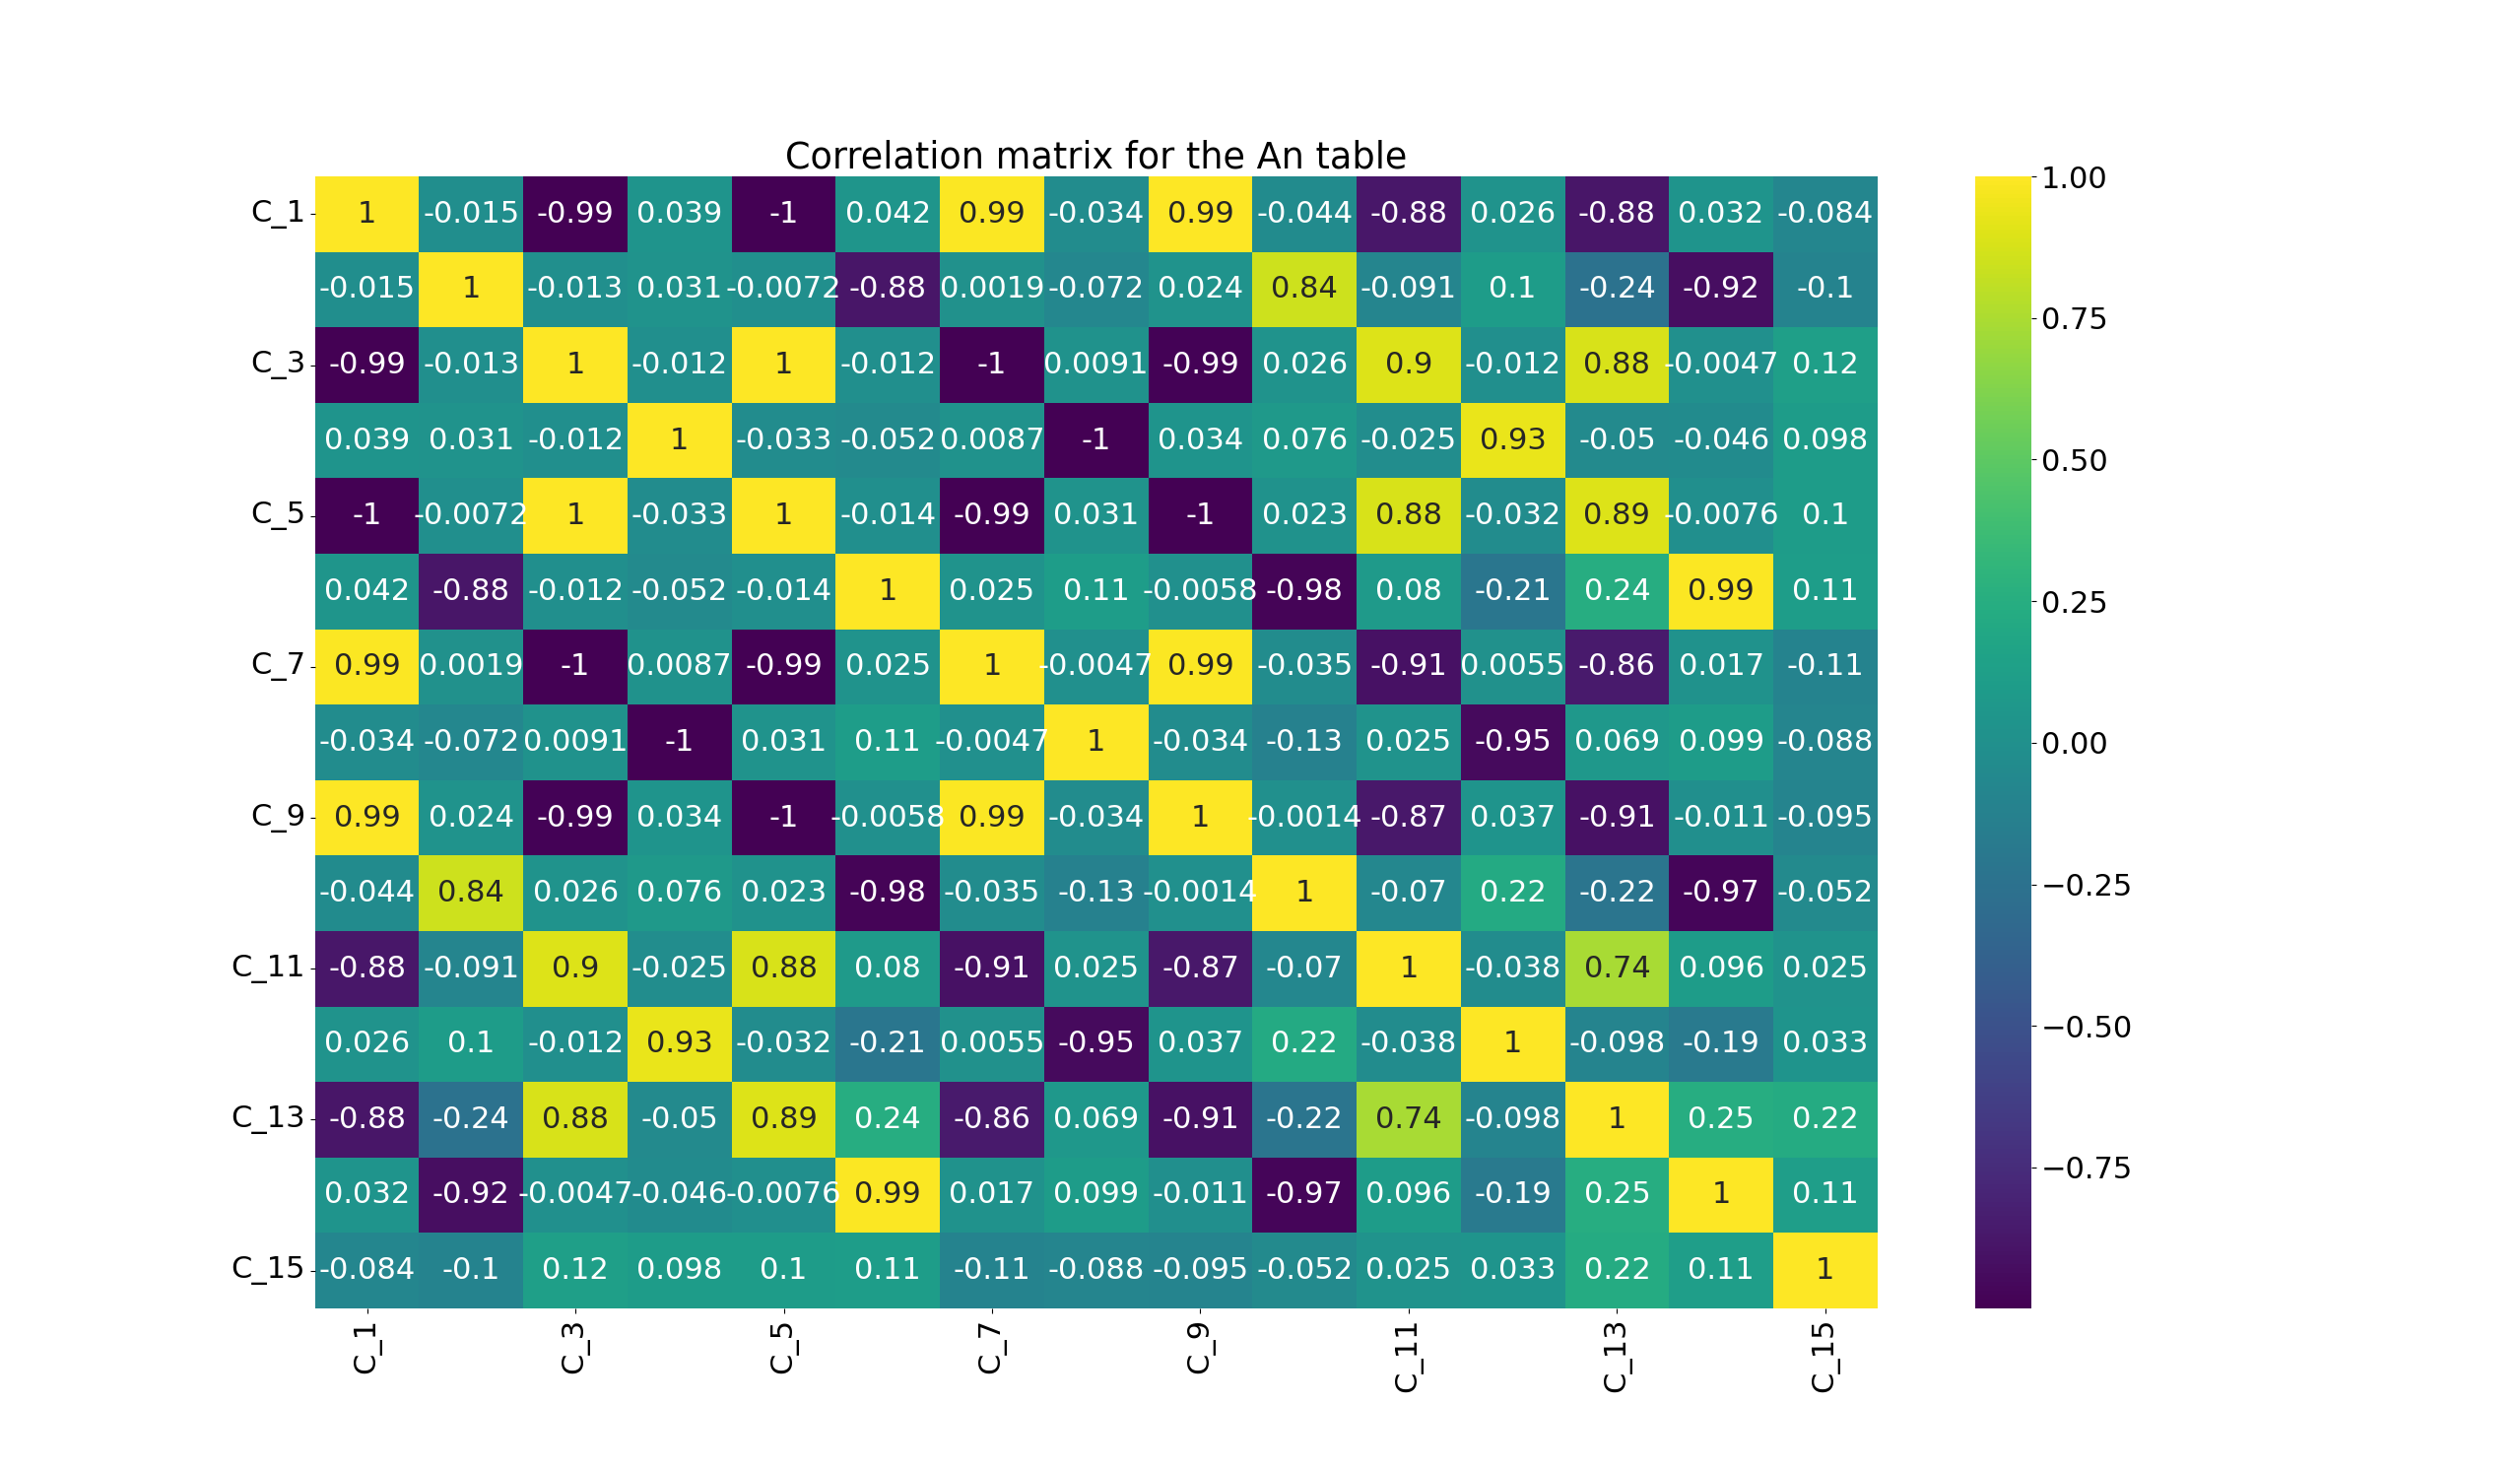
\includegraphics[width=\linewidth]{img/An_corr_matrix.png}
	\caption{The cross-correlation of the An harmonics} \label{fig:an-corr}
\end{figure}
Other than us noticing that the situation is definitely complex and doing feature extraction on this
matrix might be trickier than we would have otherwise assumed, we also noticed that Harmonic number
$2$ is strongly correlated with its odd multiples: $6, 10, 14$; which was expected behavior.

By looking at \Cref{fig:an-corr} we can gather the following information:
\begin{itemize}
	\item All the odd harmonics are strongly correlated with each other (with the sole exception
	      of harmonic $15$),
	\item Harmonic number $2$ is strongly correlated with its odd multiples,
	\item Harmonic number $4$ is strongly correlated with all its multiples,
	\item Harmonic number $15$ is the only one that is not correlated to any of the other
	      harmonics.
\end{itemize}

Keeping the information above in mind we can check \Cref{fig:an-lcorr} to understand which of the
harmonics best explain the expected results, and come up with different harmonic combinations that
should be performing at a high level.

\begin{figure}
	\centering
	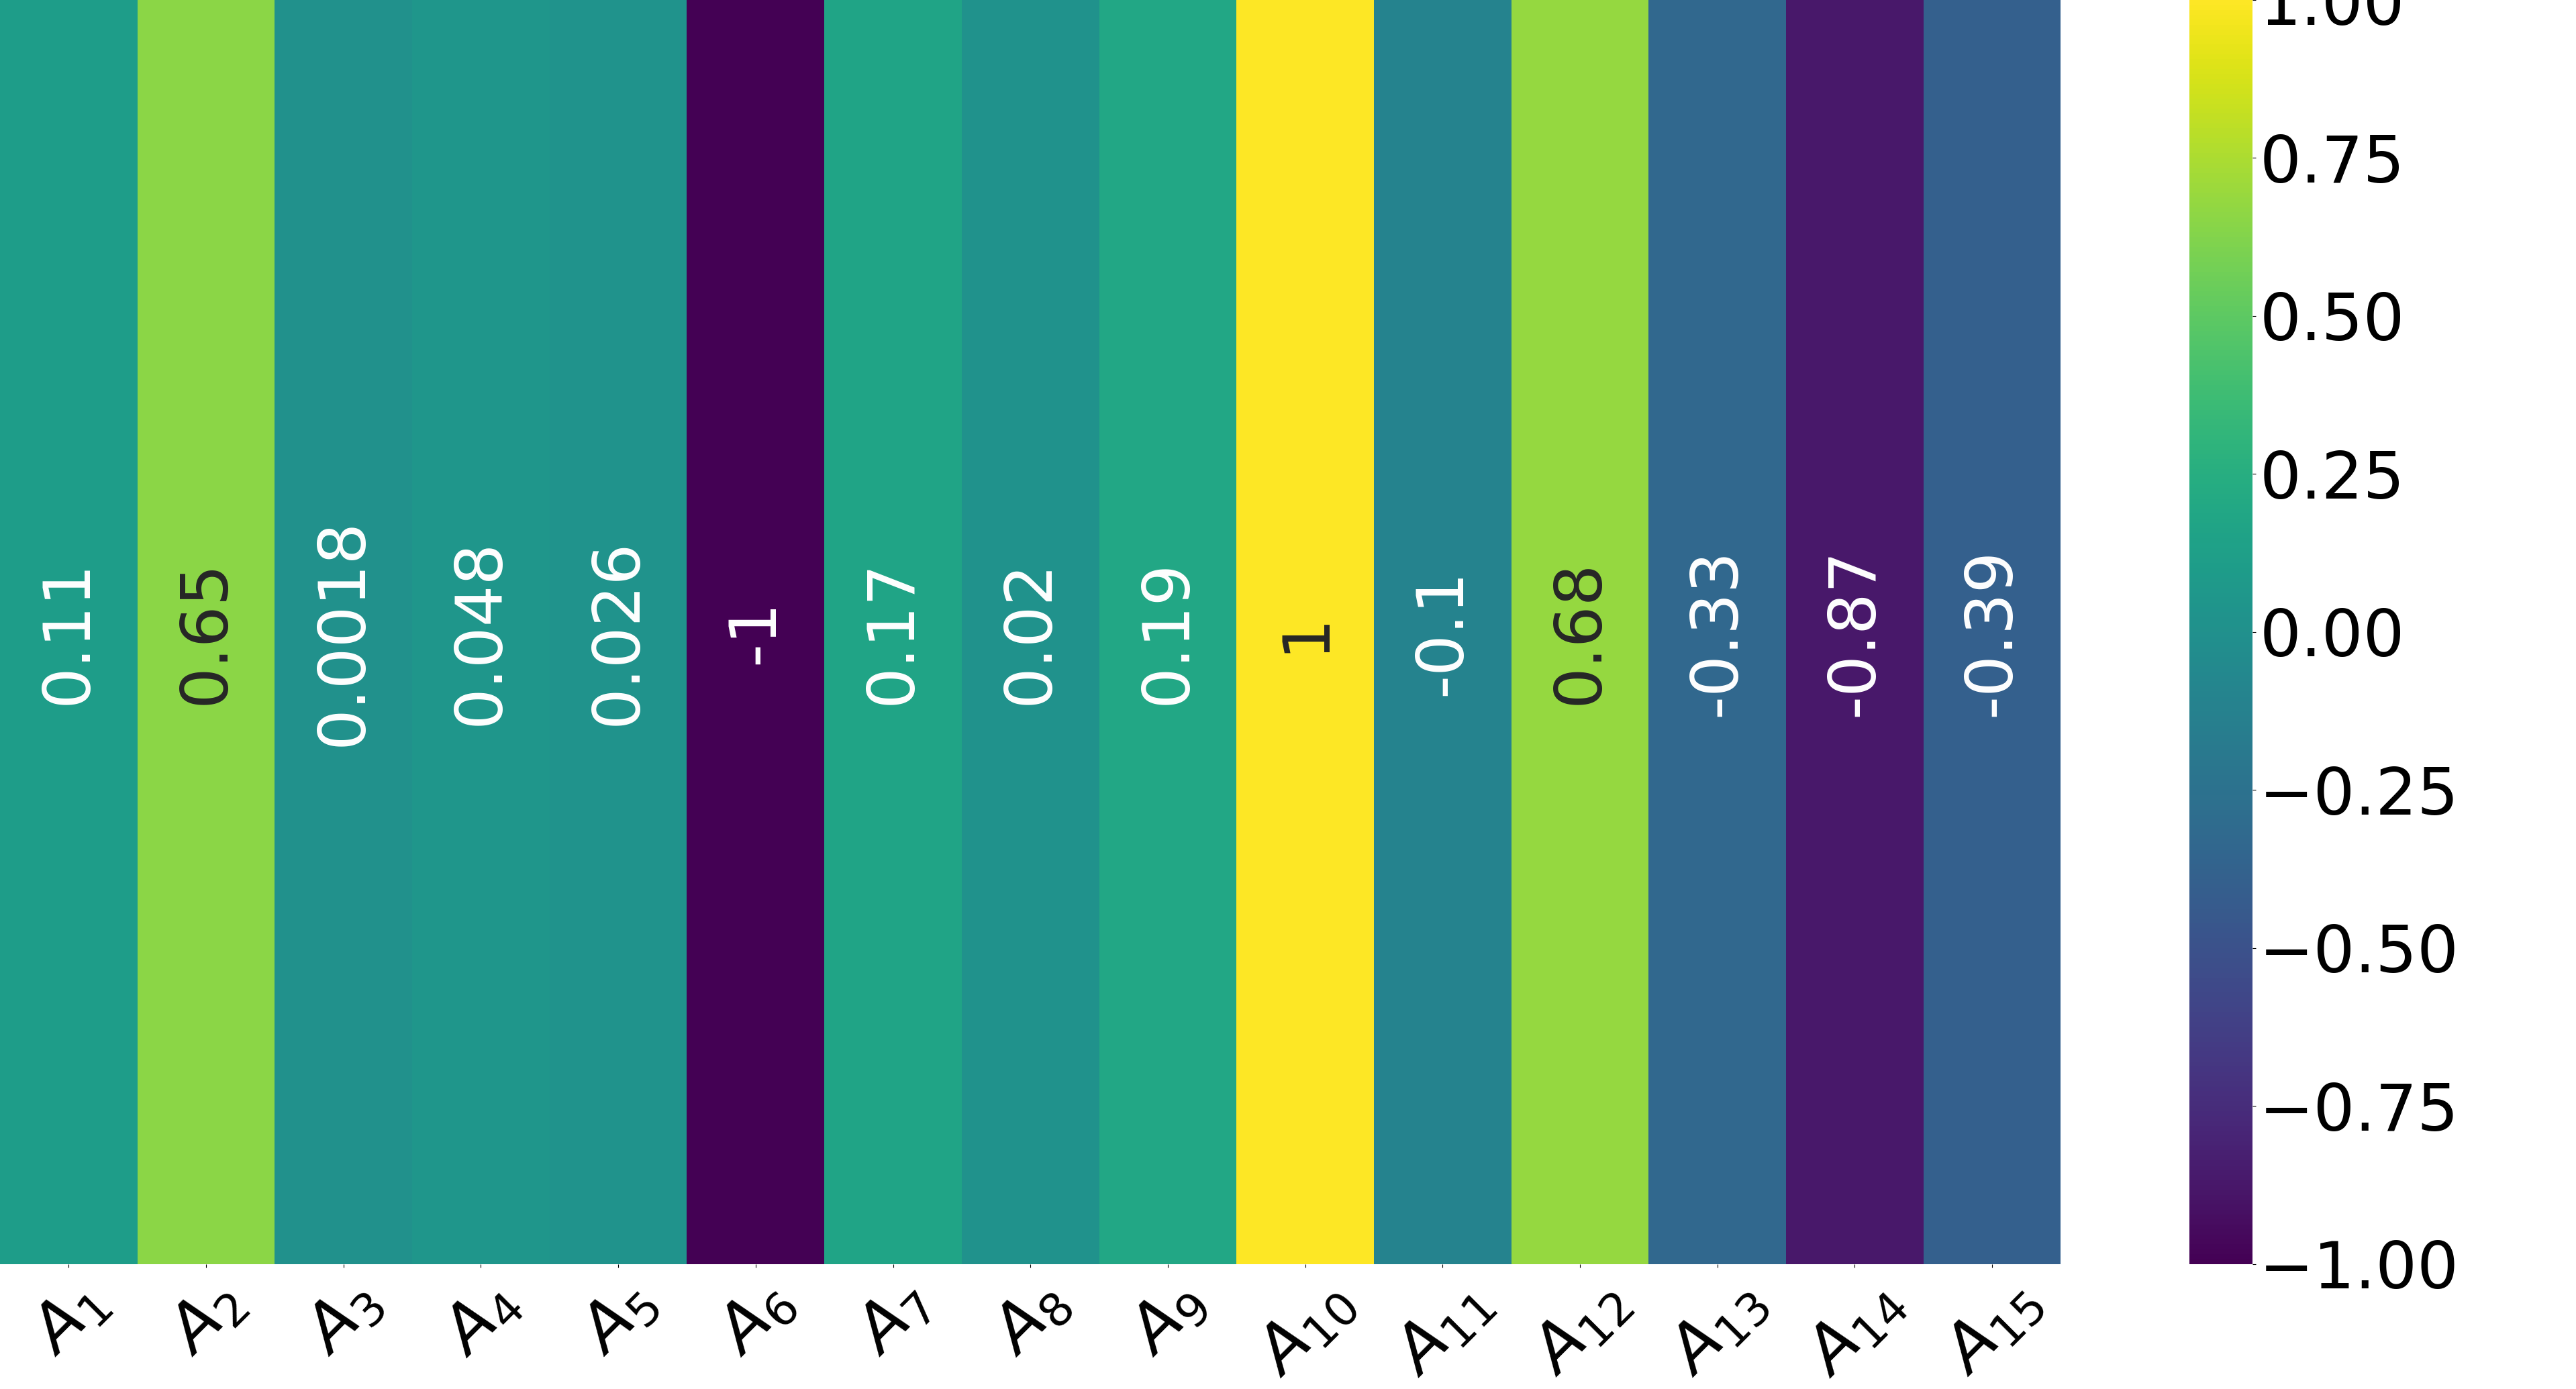
\includegraphics[width=\linewidth]{img/An_label_corr.png}
	\caption{Label correlation for the An table} \label{fig:an-lcorr}
\end{figure}

Once again, considering \Cref{fig:an-lcorr} we will be picking the harmonics with the highest label
correlation, which is identified by a higher color intensity. The result
is that harmonics number: $2, 6, 10, 11, 12, 13, 14, 15$; can explain the results very well, this
result is interesting on two sides:
\begin{enumerate}
	\item The $2^{nd}$ harmonic, as well as its odd multiples, can explain the results well, which
	      is what we expect from the theory.
	\item High order harmonics are able to explain the results better than other harmonics,
	      which is not what we would expect, since in the original analysis the value for the
	      labels was computed using primarily lower order harmonics.
\end{enumerate}
Based on all the information obtained up to this point we can conjecture that some of the best
datasets will probably contain the second harmonic, or one of its high order odd multiples, will
likely contain harmonic number $15$, as well as some other high order harmonic that doesn't collide
with anything that has been taken previously (i.e.: harmonics number $11$ or $13$). As we will see
in the following one of the best datasets that we built on this table was based on harmonics $2, 12,
	15$.

Lastly, we can check the distribution of the samples in bidimensional space, since the data have
$15$ dimensions to be able to plot them we use a dimensionality reduction technique, namely
$\textsc{pca}$ (Principal Component Analysis).
\begin{figure}[h!]
	\centering
	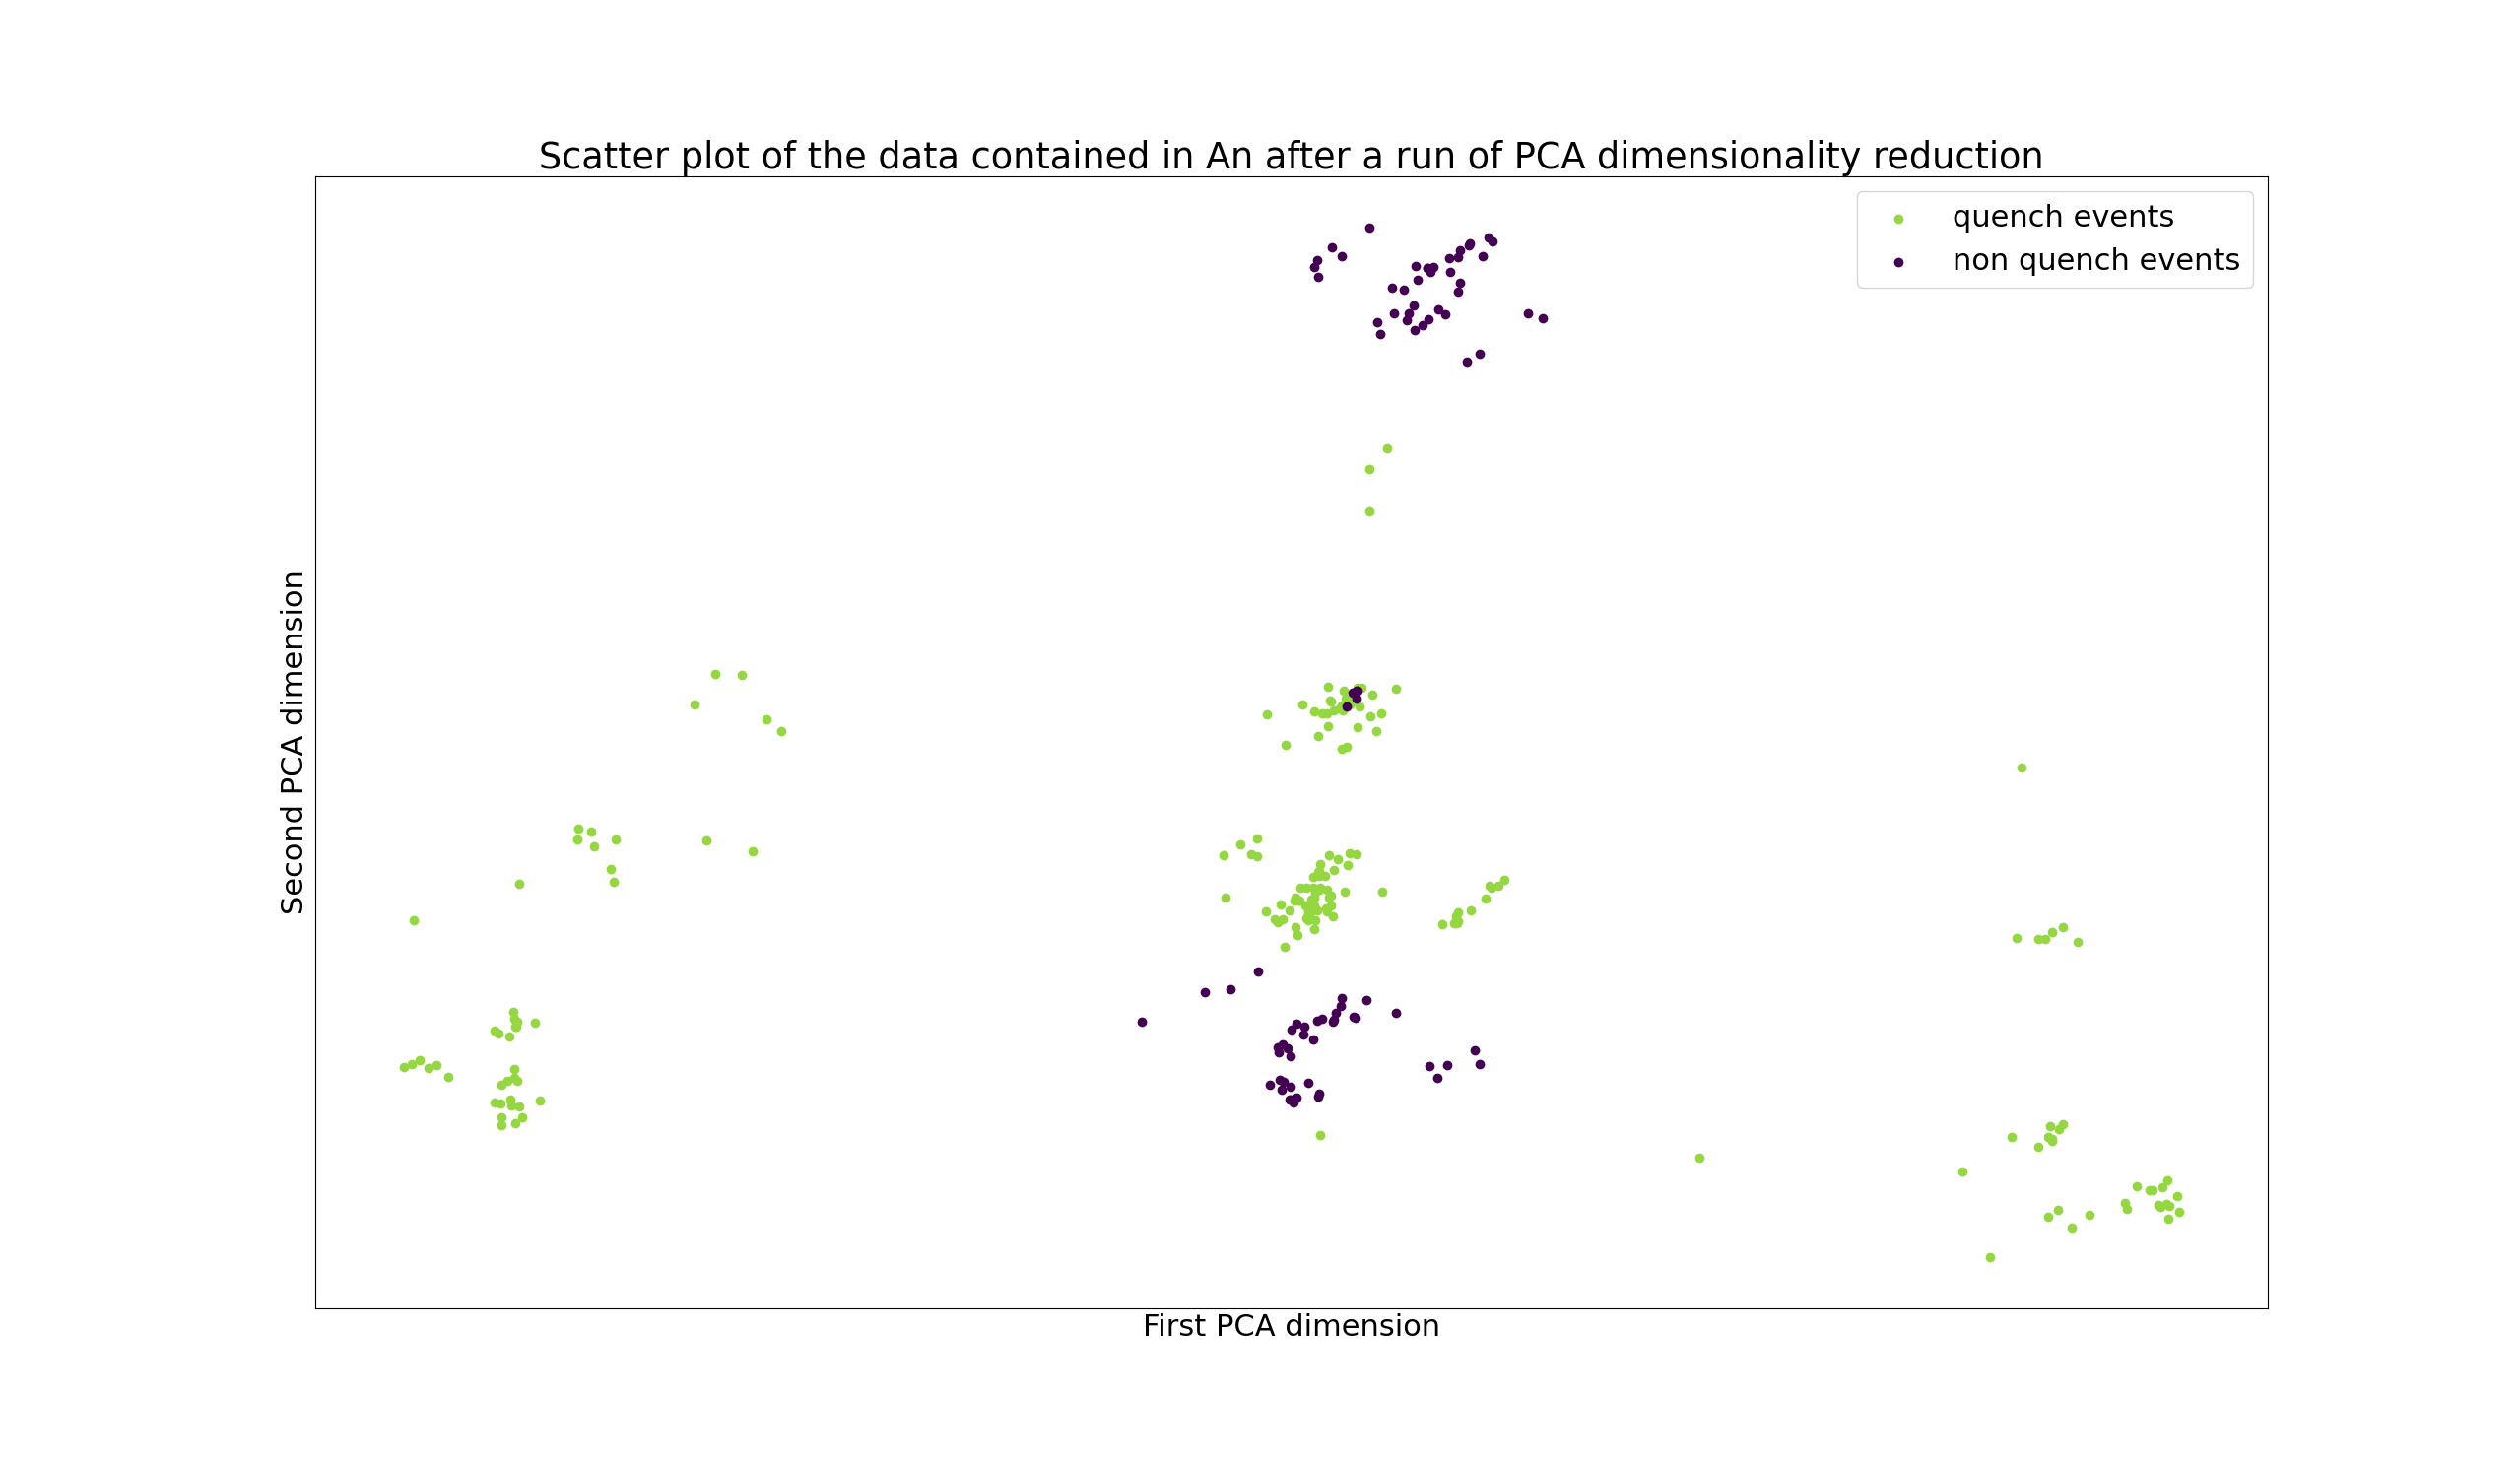
\includegraphics[width=\linewidth]{img/An_distribution.png}
	\caption{Data distribution for the An table after applying $\textsc{pca}$ dimensionality
		reduction} \label{fig:an-dist}
\end{figure}

It can be seen in \Cref{fig:an-dist} that the samples, after dimensionality reduction, are distributed very nicely in a series
of zones, each zone has a very high degree of purity. The very good distribution of the samples is
very likely the reason why the models built on this table are performing so well.

\subsubsection{Bn table}
We can use a similar procedure on the Bn table, which in most of the tests proved to be the worst
table to use to build models with, this is likely due, if we look at \Cref{fig:bn-dist}, to the very
poor distribution of the data, as we can see it's really hard to find a way to separate the central
portion of the data, and this difficulty will be reflected in the performance of most models that
will be introduced in this chapter.
\begin{figure}[h!]
	\centering
	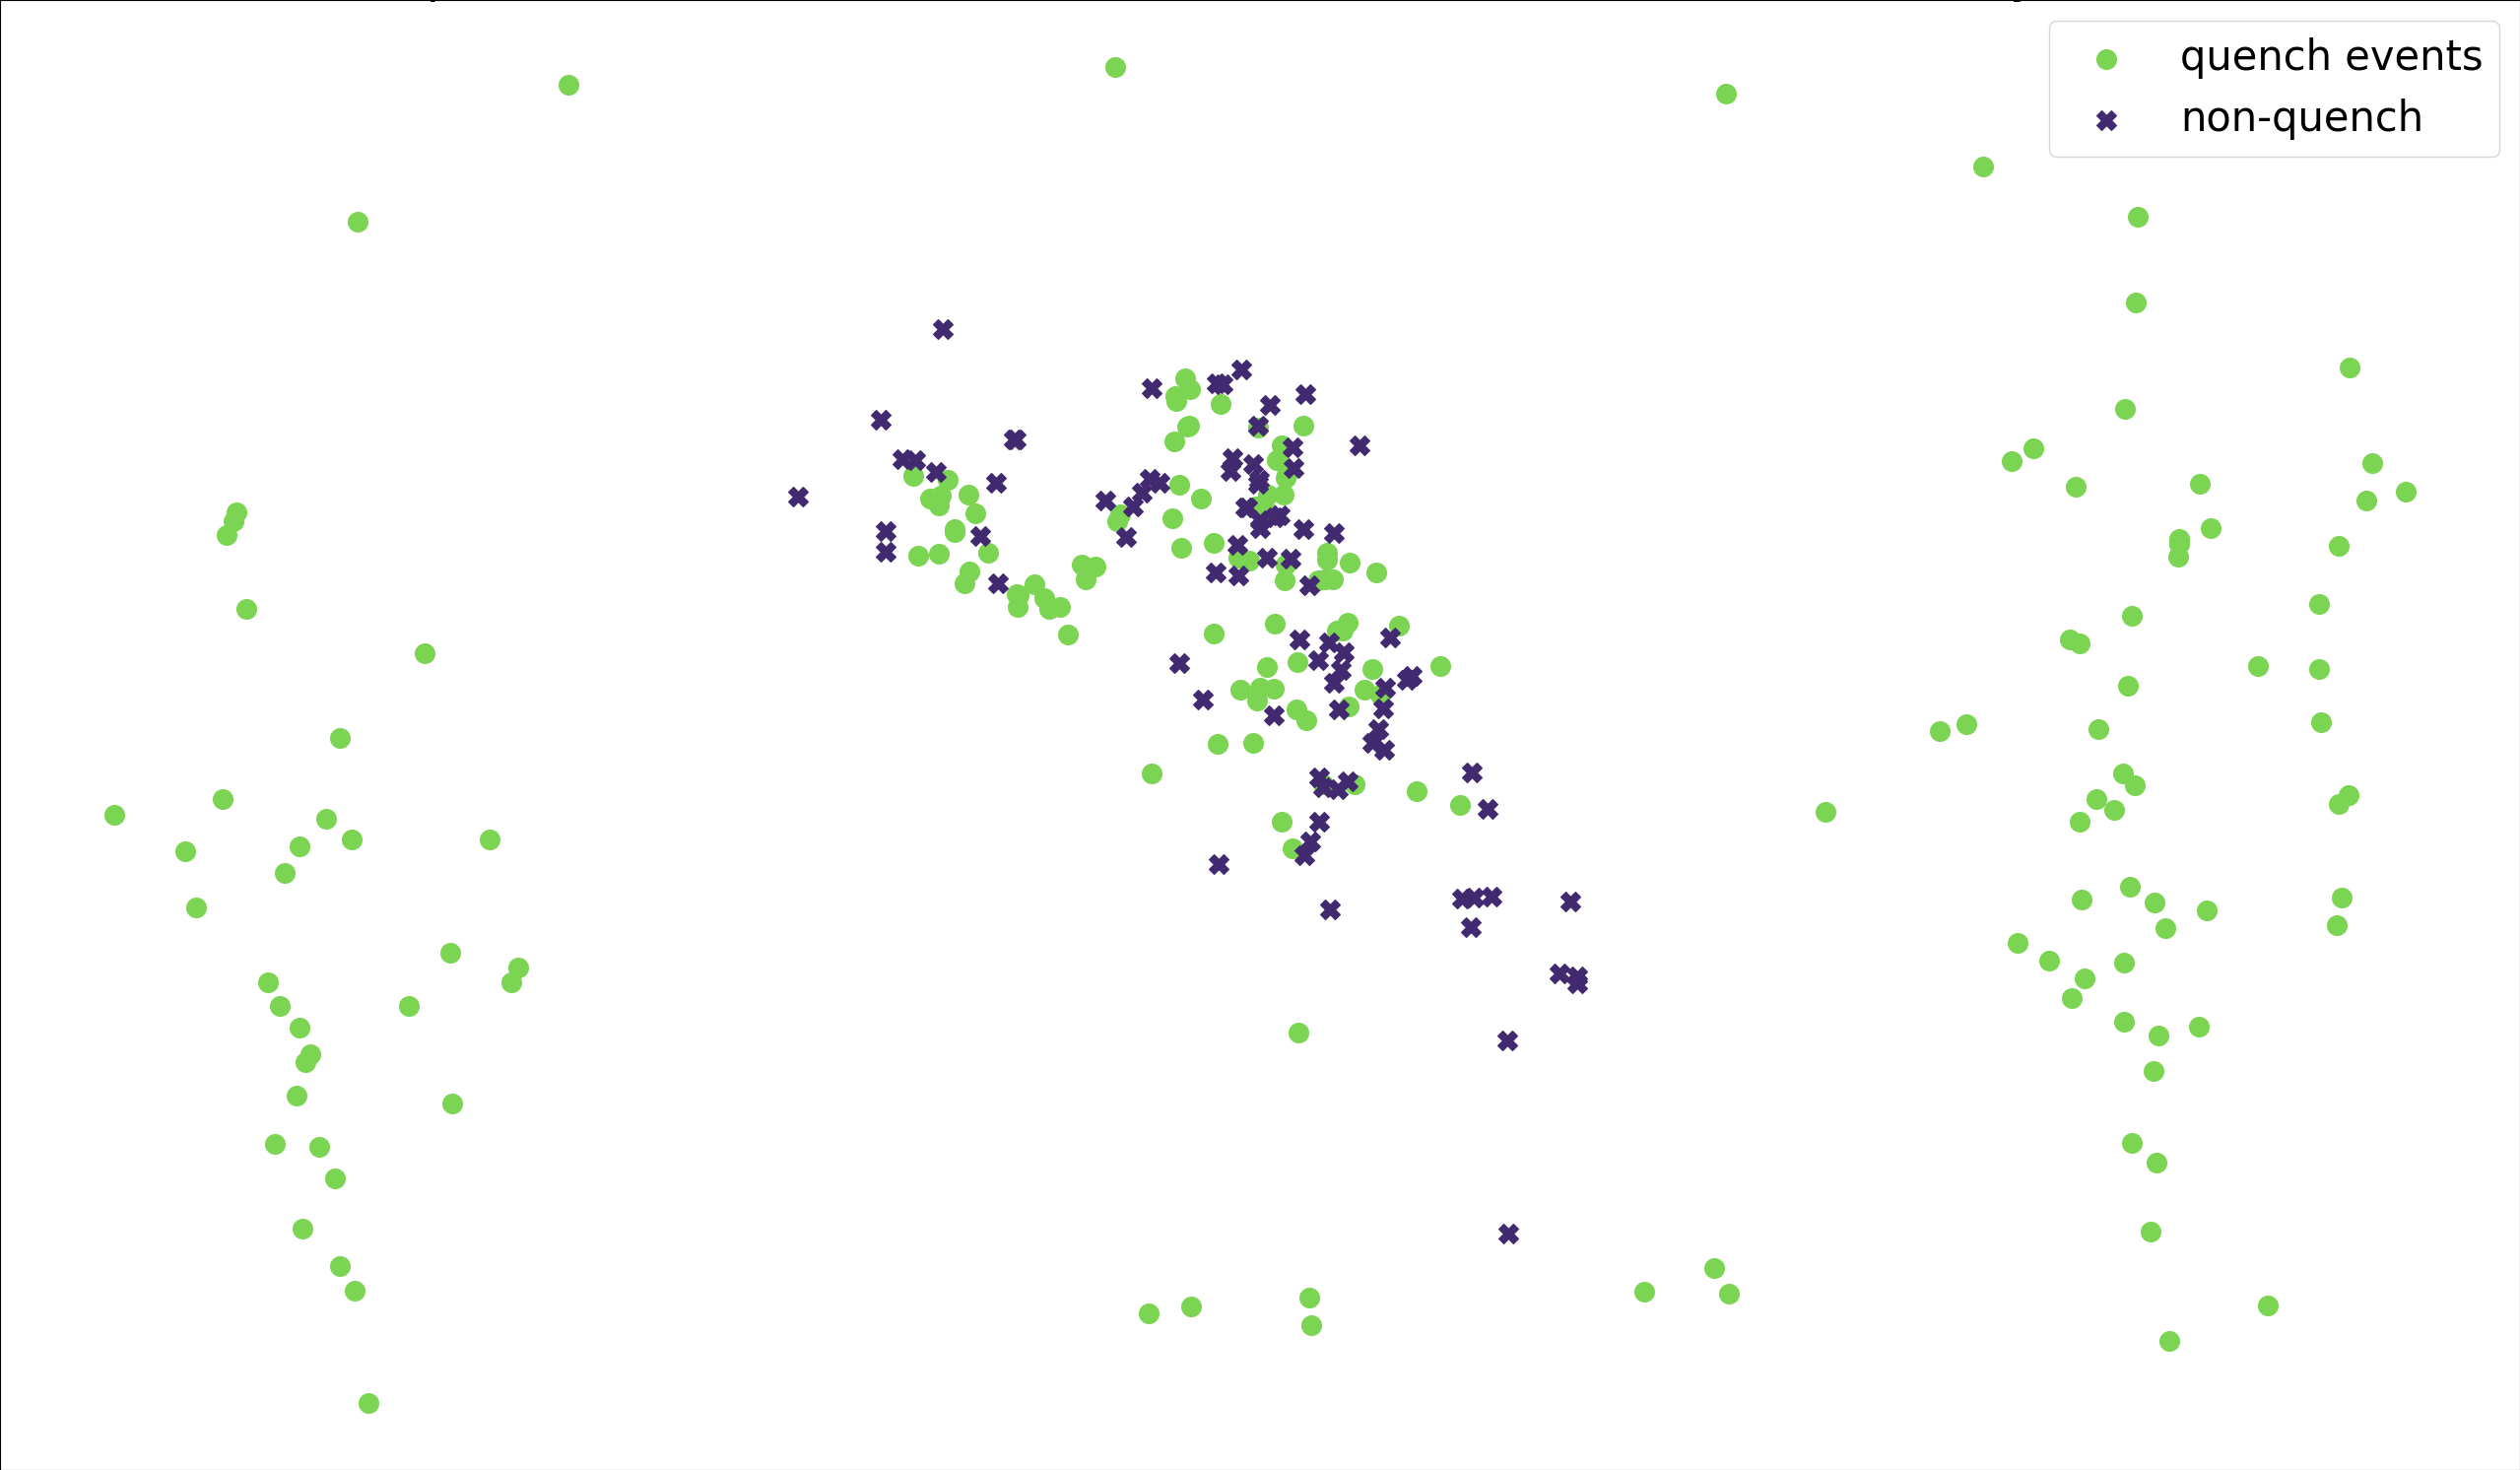
\includegraphics[width=\linewidth]{img/Bn_distribution.png}
	\caption{Data distribution for the Bn table after applying $\textsc{pca}$ dimensionality
		reduction} \label{fig:bn-dist}
\end{figure}

As we did for An we check the cross-correlation of the Bn table, and the results are actually very
similar.
\begin{figure}[h!]
	\centering
	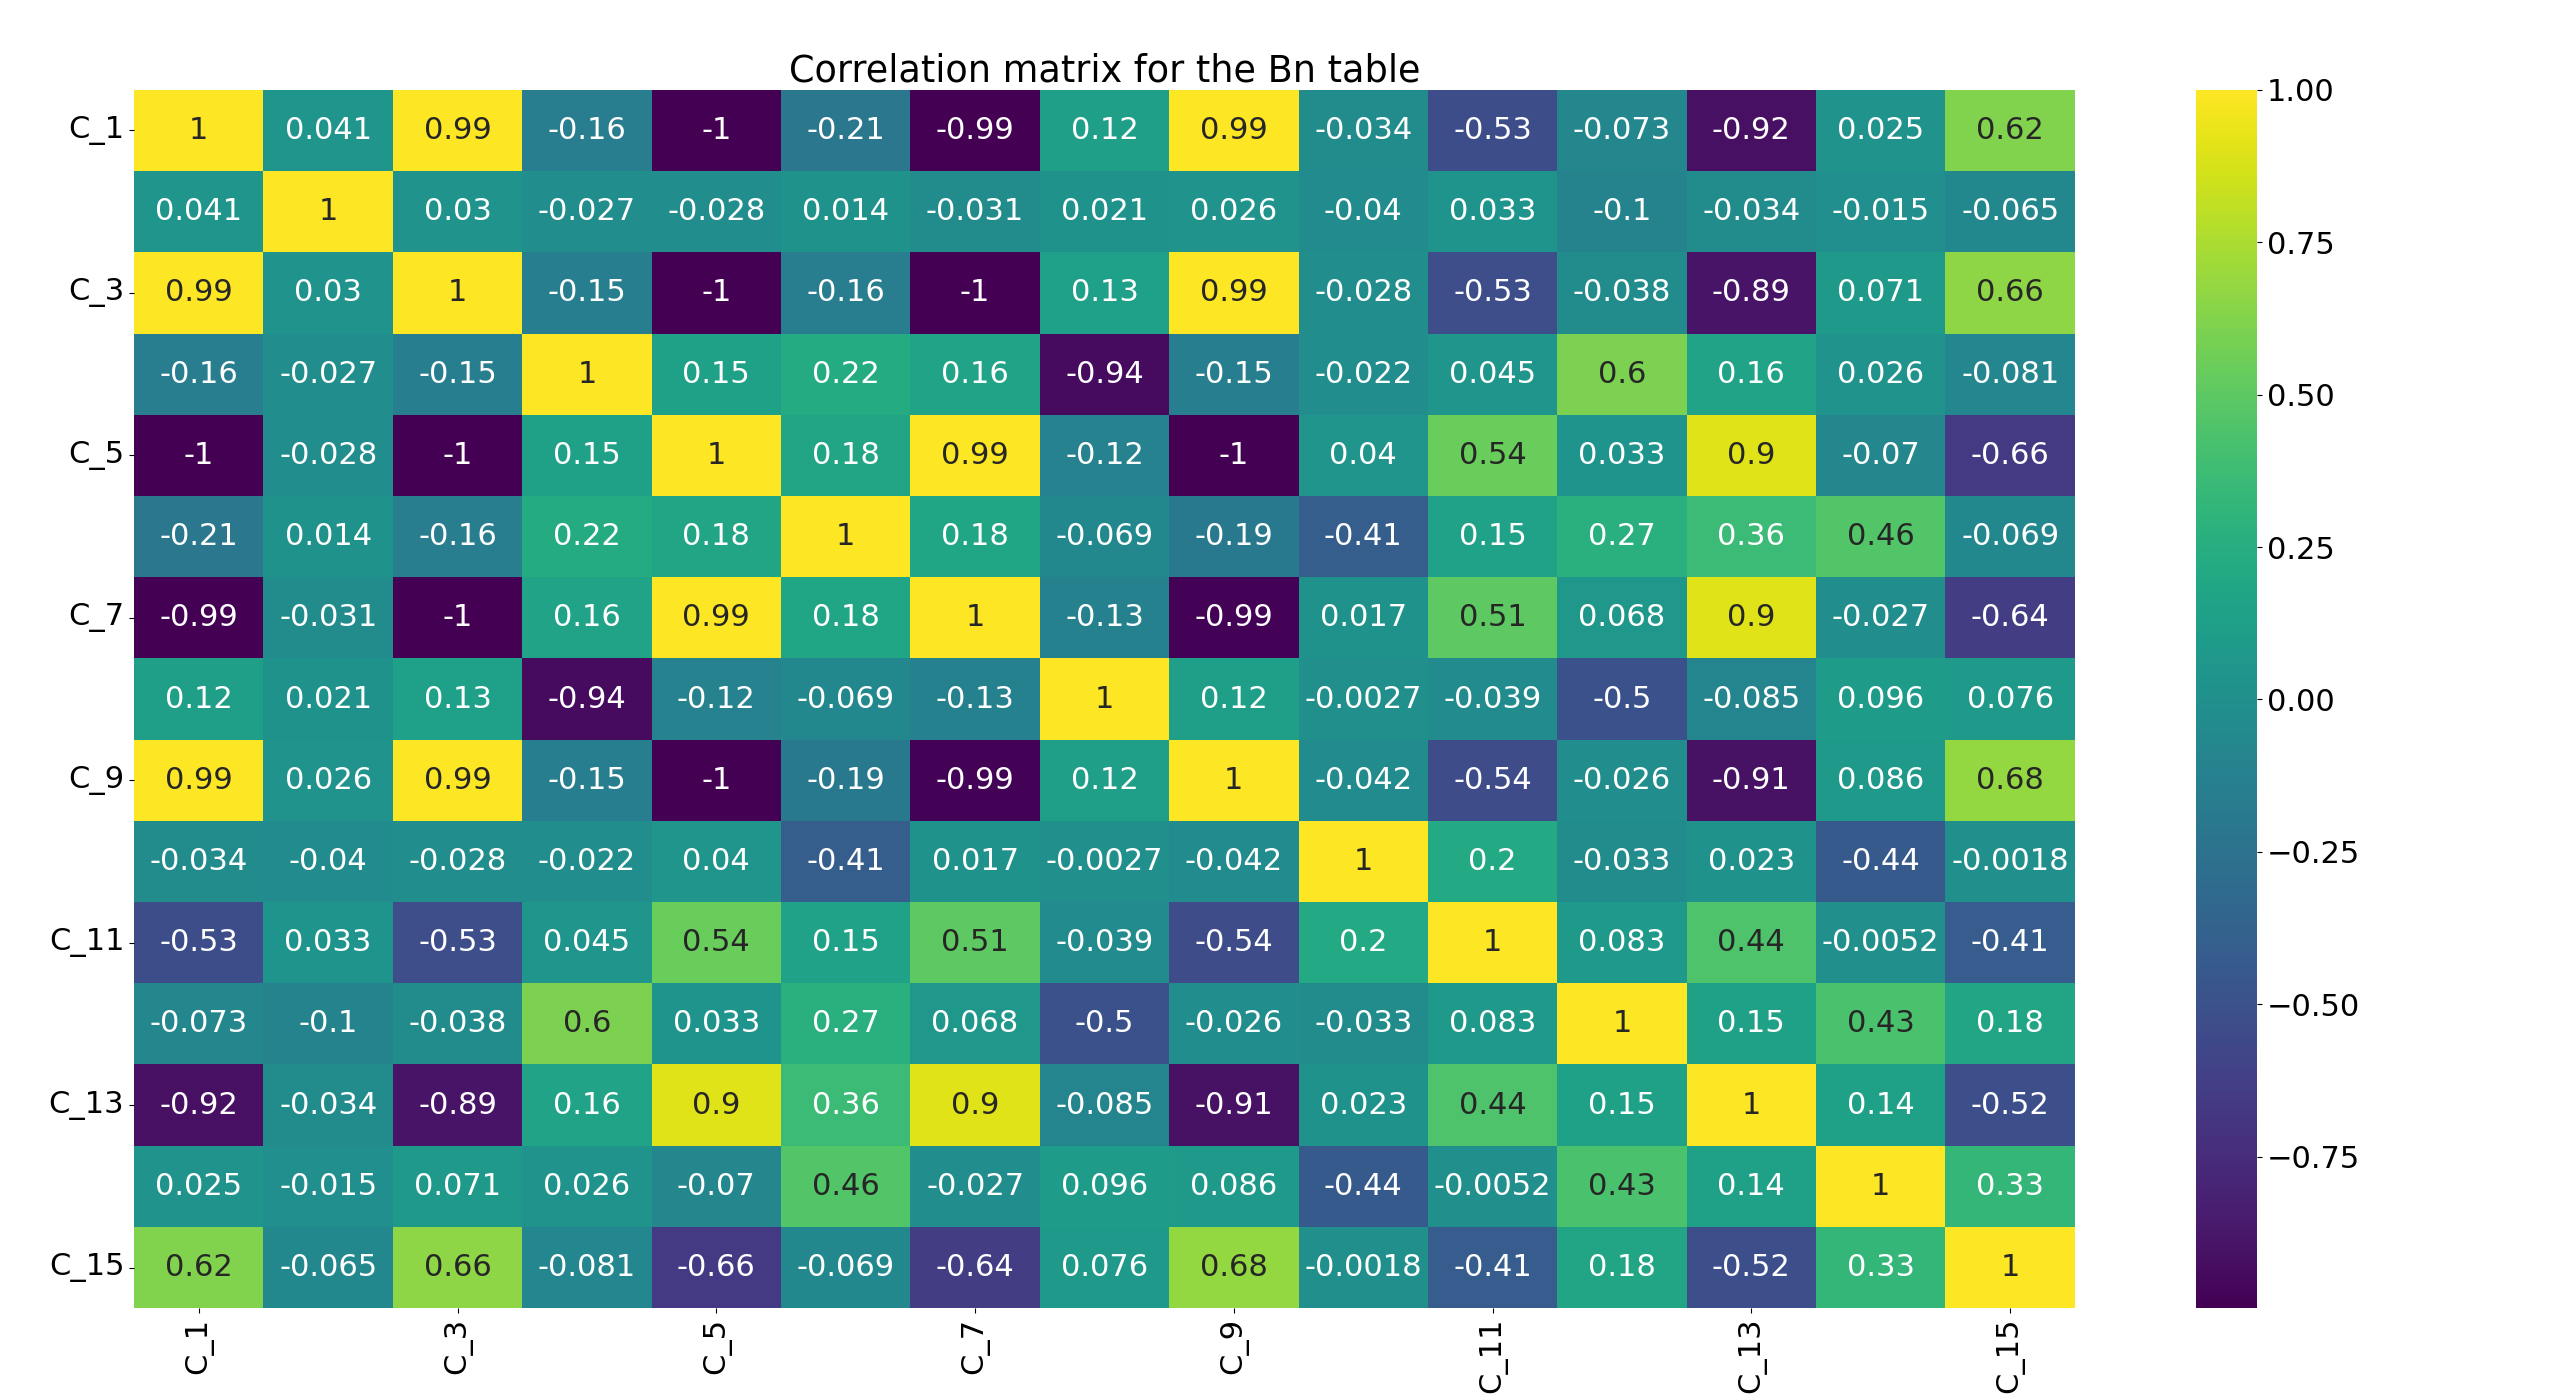
\includegraphics[width=\linewidth]{img/Bn_corr_matrix.png}
	\caption{The cross-correlation of the Bn harmonics} \label{fig:bn-corr}
\end{figure}
Possibly the biggest difference between \Cref{fig:an-corr} and \Cref{fig:bn-corr}, apart from the
obvious different in the value of the correlation coefficient, we can see that harmonic $2$ is not
strongly correlated with any other harmonic anymore, and harmonic number $15$ has a discrete
correlation with all odd harmonics.

If we check the correlation of the harmonics with the labels (\Cref{fig:bn-lcorr}), we can see that, apparently, almost all
harmonic have a good enough correlation with the solution, but despite this, the performance of all
models built on Bn suffered.
\begin{figure}
	\centering
	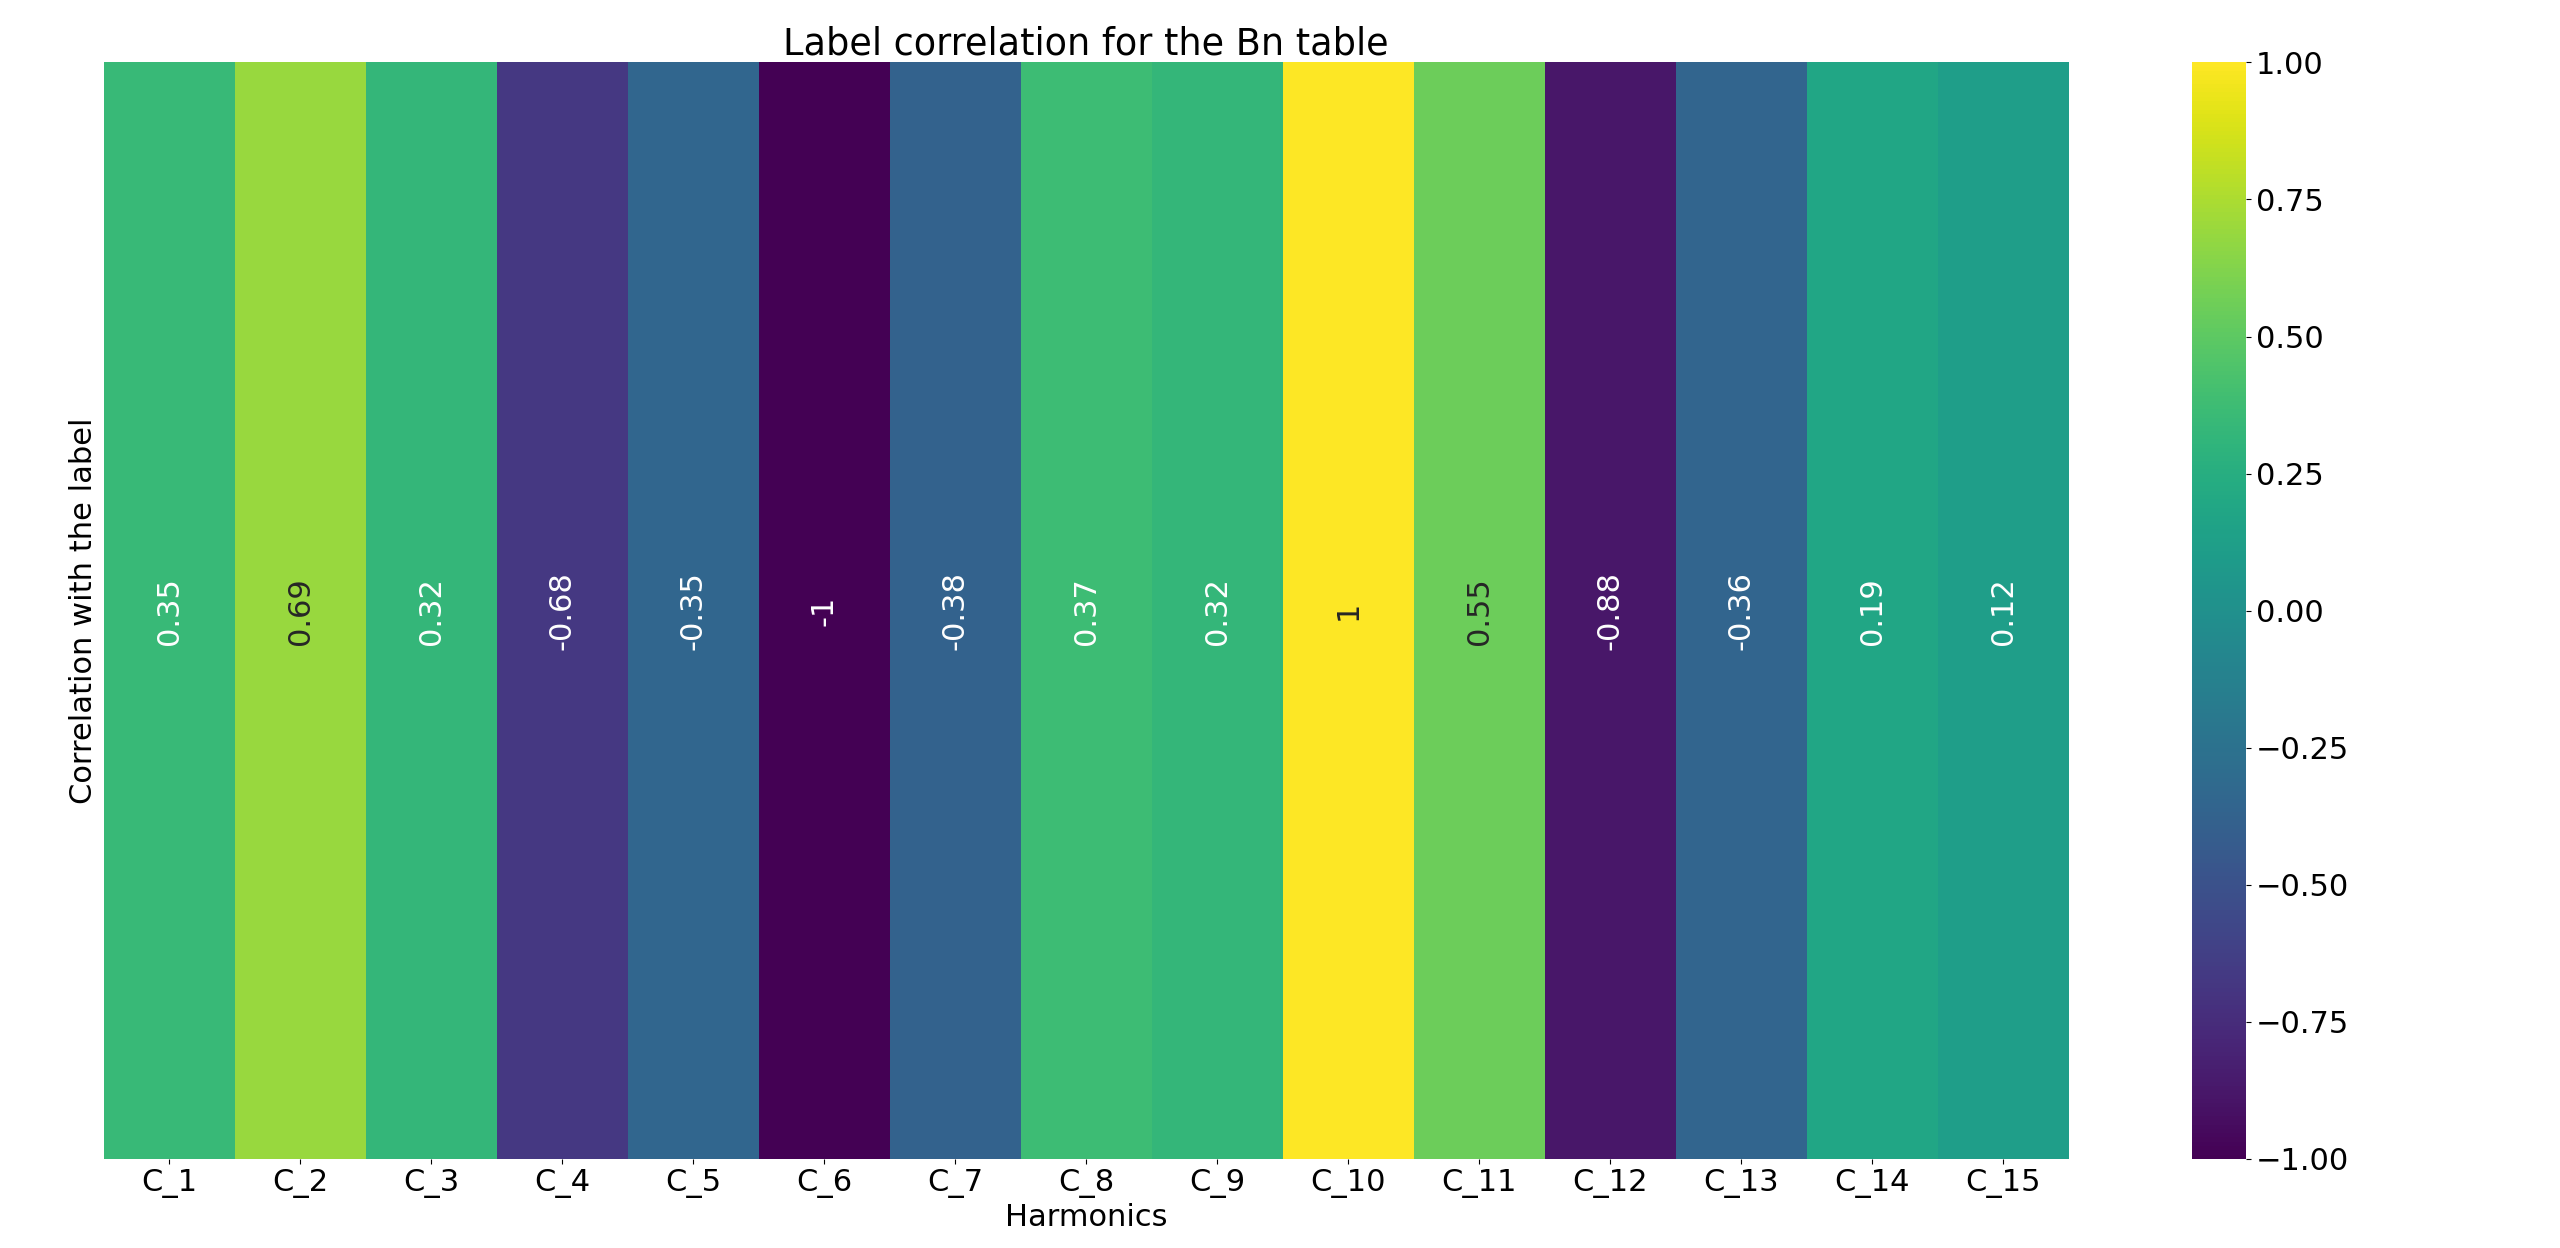
\includegraphics[width=\linewidth]{img/Bn_label_corr.png}
	\caption{Label correlation for the Bn table} \label{fig:bn-lcorr}
\end{figure}

\subsubsection{Cnmod table}
The Cnmod table combines the information present in An and Bn, as we saw in the previous section,
while the An table seems to be very good and has a very promising topology, the Bn table has a
central 'cluster' of data with a high degree of impurity, where 'non-quench' and 'quench' samples
mix and seem to be hardly separable.

Cnmod was expected to be one of the best tables to solve the problem, but as we will see in future
sections, it consistently falls short of the An table, and that is most likely due to the
introduction of the information carried by Bn.
\begin{figure}[h!]
	\centering
	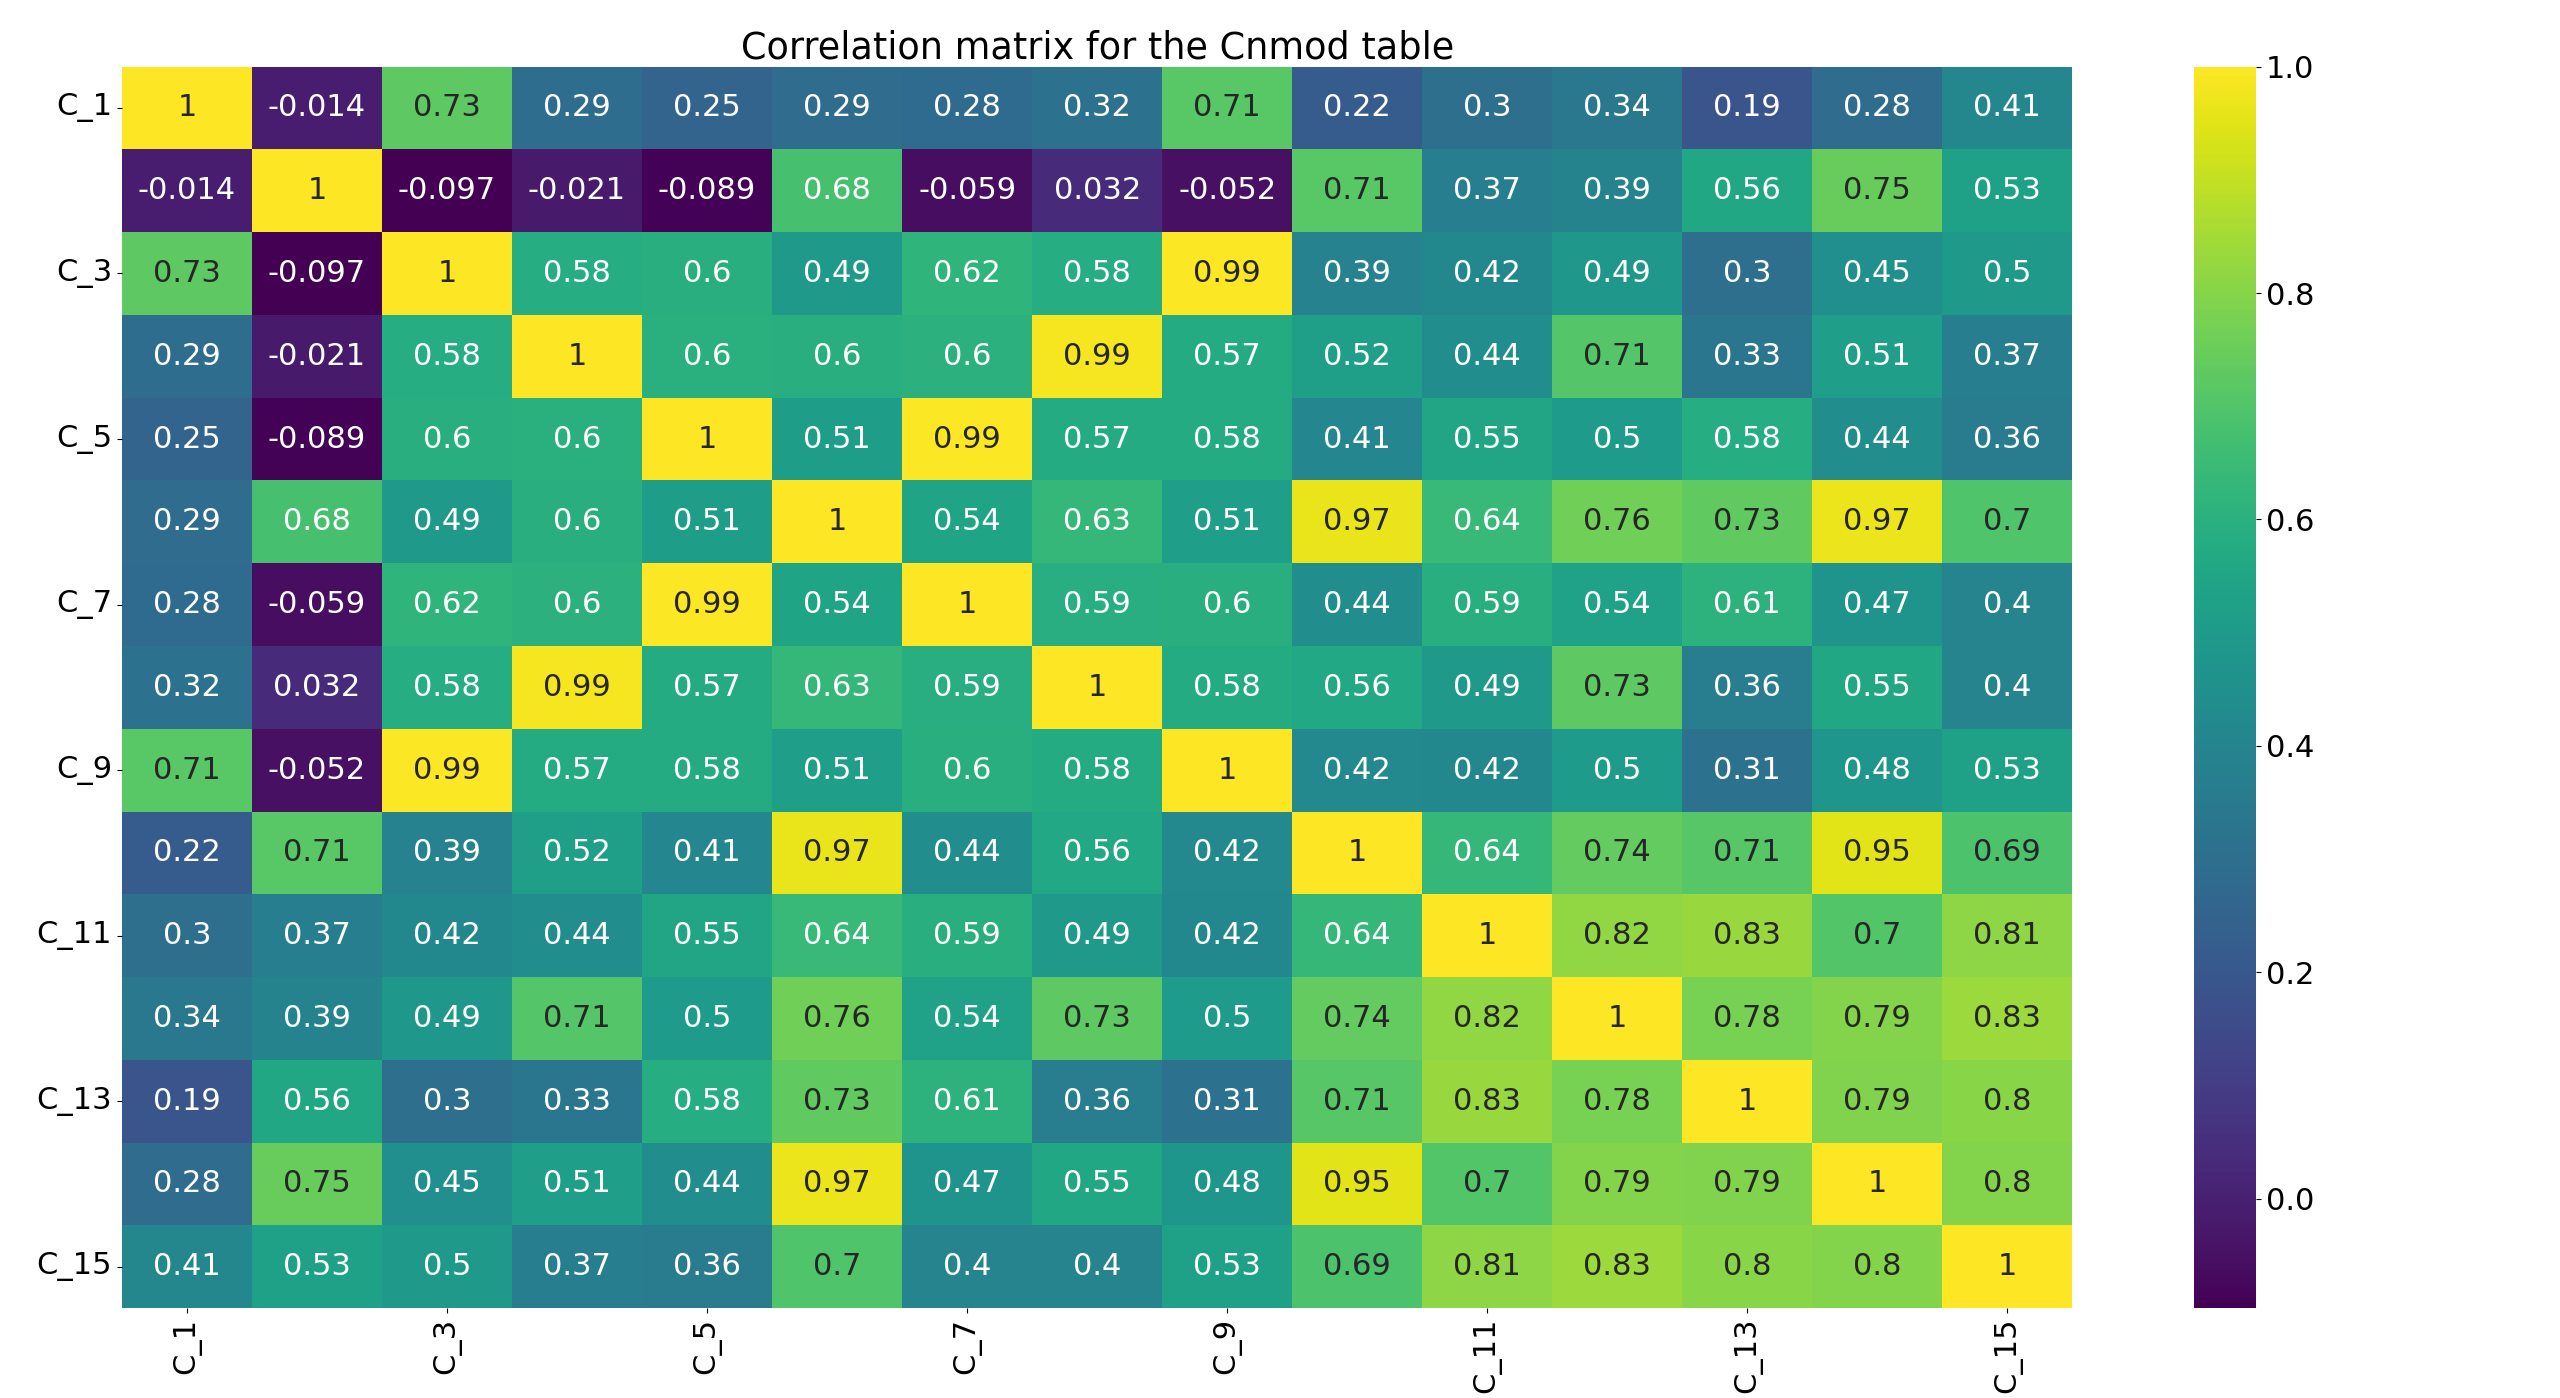
\includegraphics[width=\linewidth]{img/Cnmod_corr_matrix.png}
	\caption{The cross-correlation of the Cnmod harmonics} \label{fig:cnmod-corr}
\end{figure}

As we can see in \Cref{fig:cnmod-corr} the correlation matrix for Cnmod is very complicated,
harmonic number $2$ can explain basically any other harmonic until number $9$ and harmonics between
$10$ and $15$ have a medium correlation with each other. We can add to this the fact that harmonic
number $4$ is strongly correlated with its multiples and the result is that picking an harmonic
composition that is not, at least discretely, correlated in some way is extremely tricky.

If we check the correlation between the harmonics and the labels \Cref{fig:cnmod-lcorr} we can see
that the first harmonics explain really well the expected results.
\begin{figure}[h!]
	\centering
	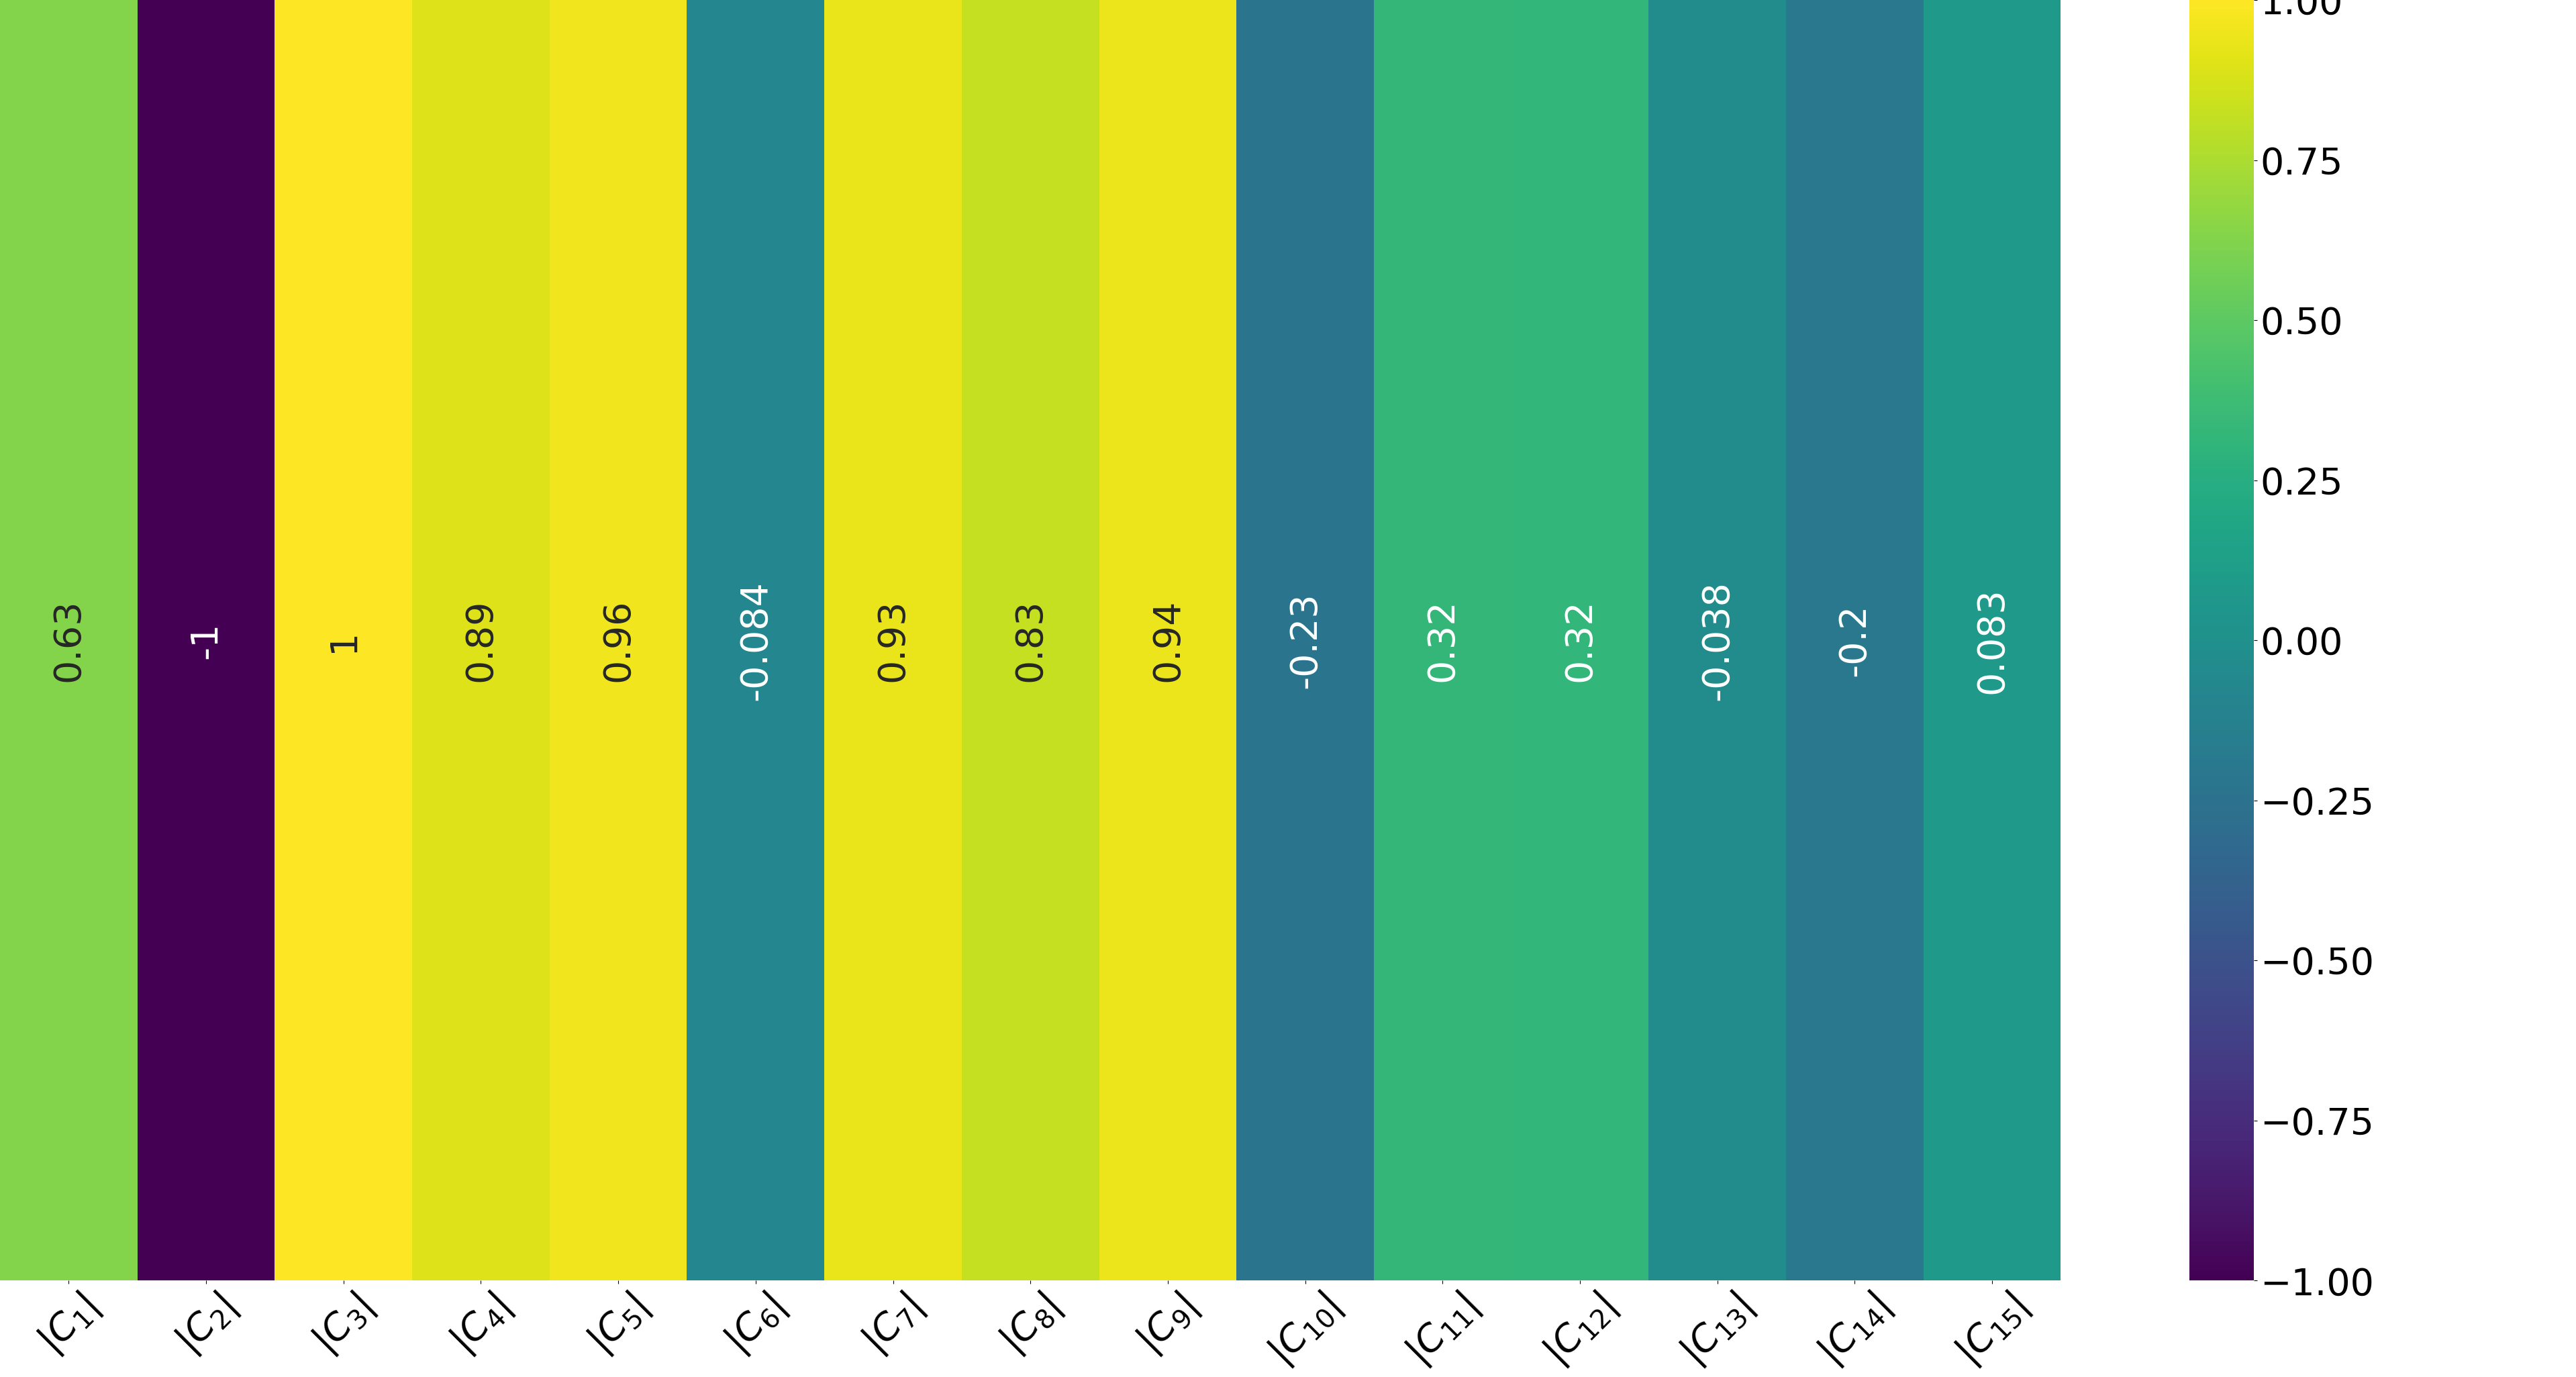
\includegraphics[width=\linewidth]{img/Cnmod_label_corr.png}
	\caption{Label correlation for the Cnmod table} \label{fig:cnmod-lcorr}
\end{figure}

Looking at both \Cref{fig:cnmod-corr} and \Cref{fig:cnmod-lcorr}, we can conclude that two different
routs could be pursued:
\begin{itemize}
	\item If harmonic number $2$ carries enough information it can be used in alongside one or
	      more high-order harmonics,
	\item Another route possible is to use harmonic number $3$ and some other low-order
	      harmonics (potentially even the first one) alongside one low-order harmonic (e.g.,
	      $14$).
\end{itemize}
As we will see in a future section the choice that yielded the better performance is to use a
dataset based on harmonic $3$.

Before considering the last table let us stop once again to check the distribution of the
dimensionality reduction for Cnmod.
\begin{figure}[h!]
	\centering
	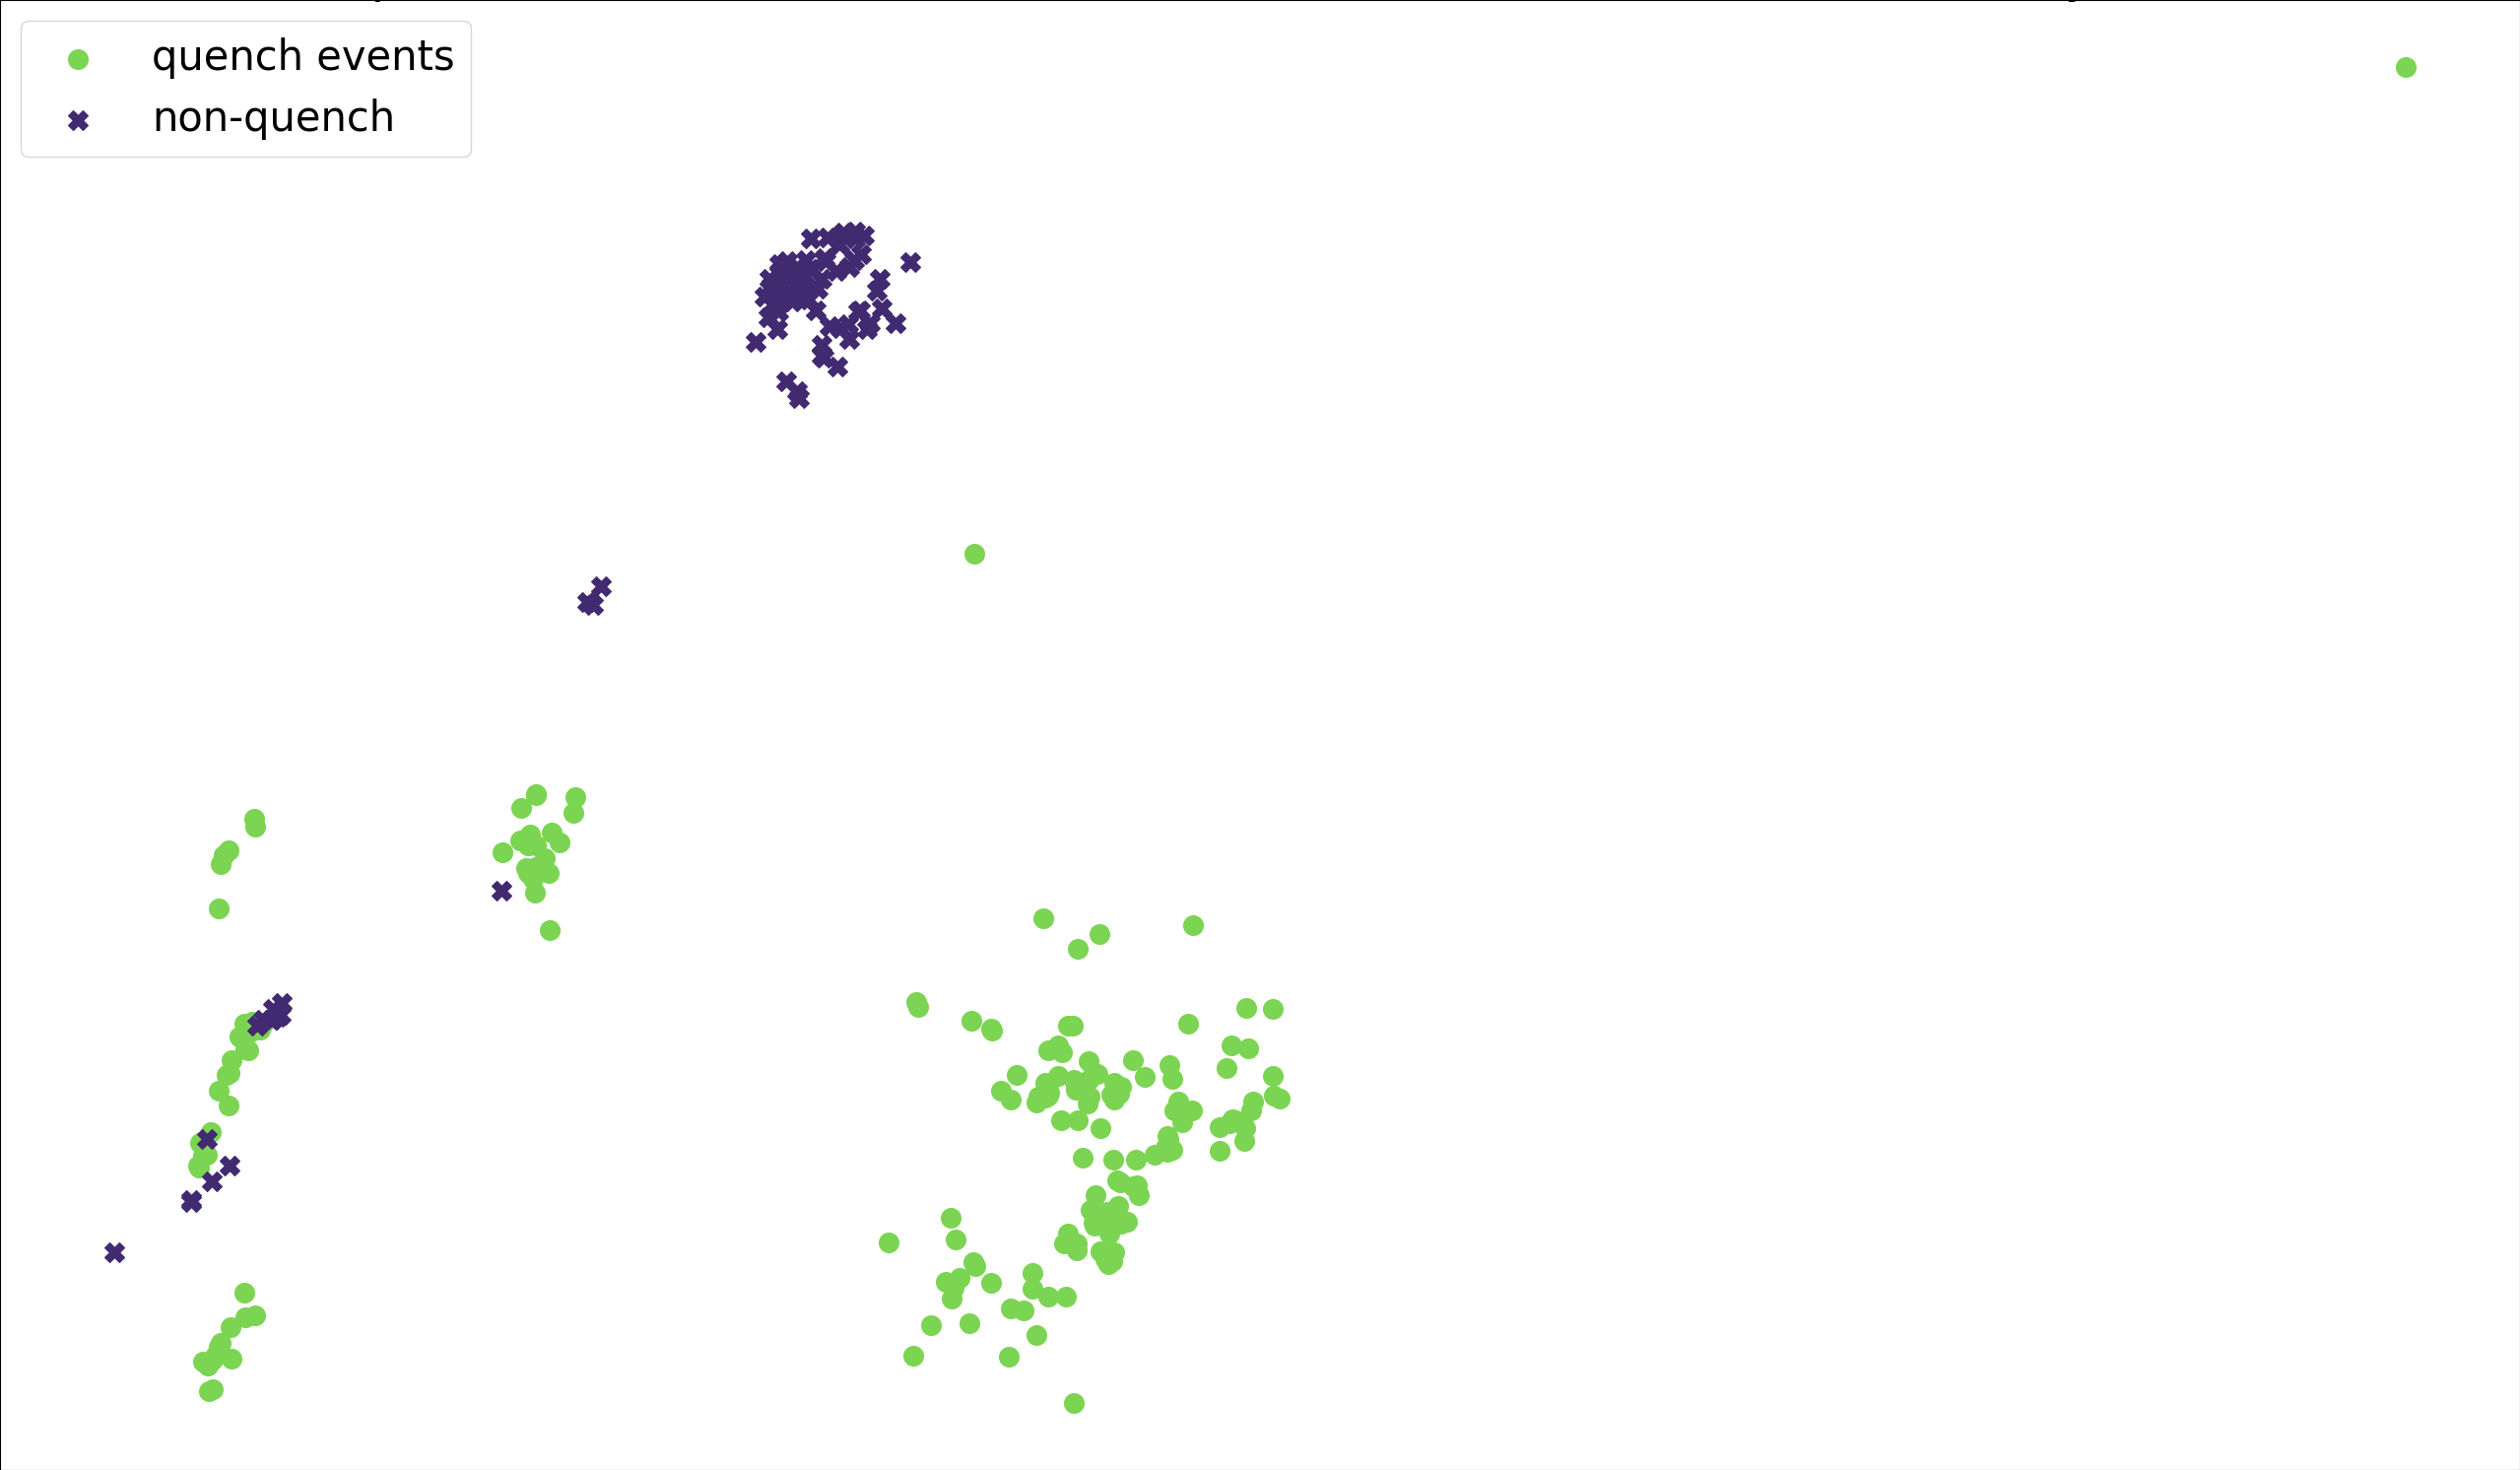
\includegraphics[width=\linewidth]{img/Cnmod_distribution.png}
	\caption{Data distribution for the Cnmod table after applying $\textsc{pca}$ dimensionality
		reduction} \label{fig:cnmod-dist}
\end{figure}
As we can see in \Cref{fig:cnmod-dist} the samples are characterized by a good enough distribution,
we could easily identify clusters with a high degree of purity, apart from the one in the leftmost
region of the image, which contains many points tagged as quench events and many points tagged as
non quenches.

\subsubsection{Phi table}
As we will see in further sections the Phi table did not perform exceptionally, but it consistently
outperformed the one based on Bn. I believe that, as we saw with Bn, the root of the bad performance
is standing in the fact that both tables have a high degree of homogeneity in the distribution of
the samples, this can be seen quite clearly in \Cref{fig:phi-dist}.

\begin{figure}[h!]
	\centering
	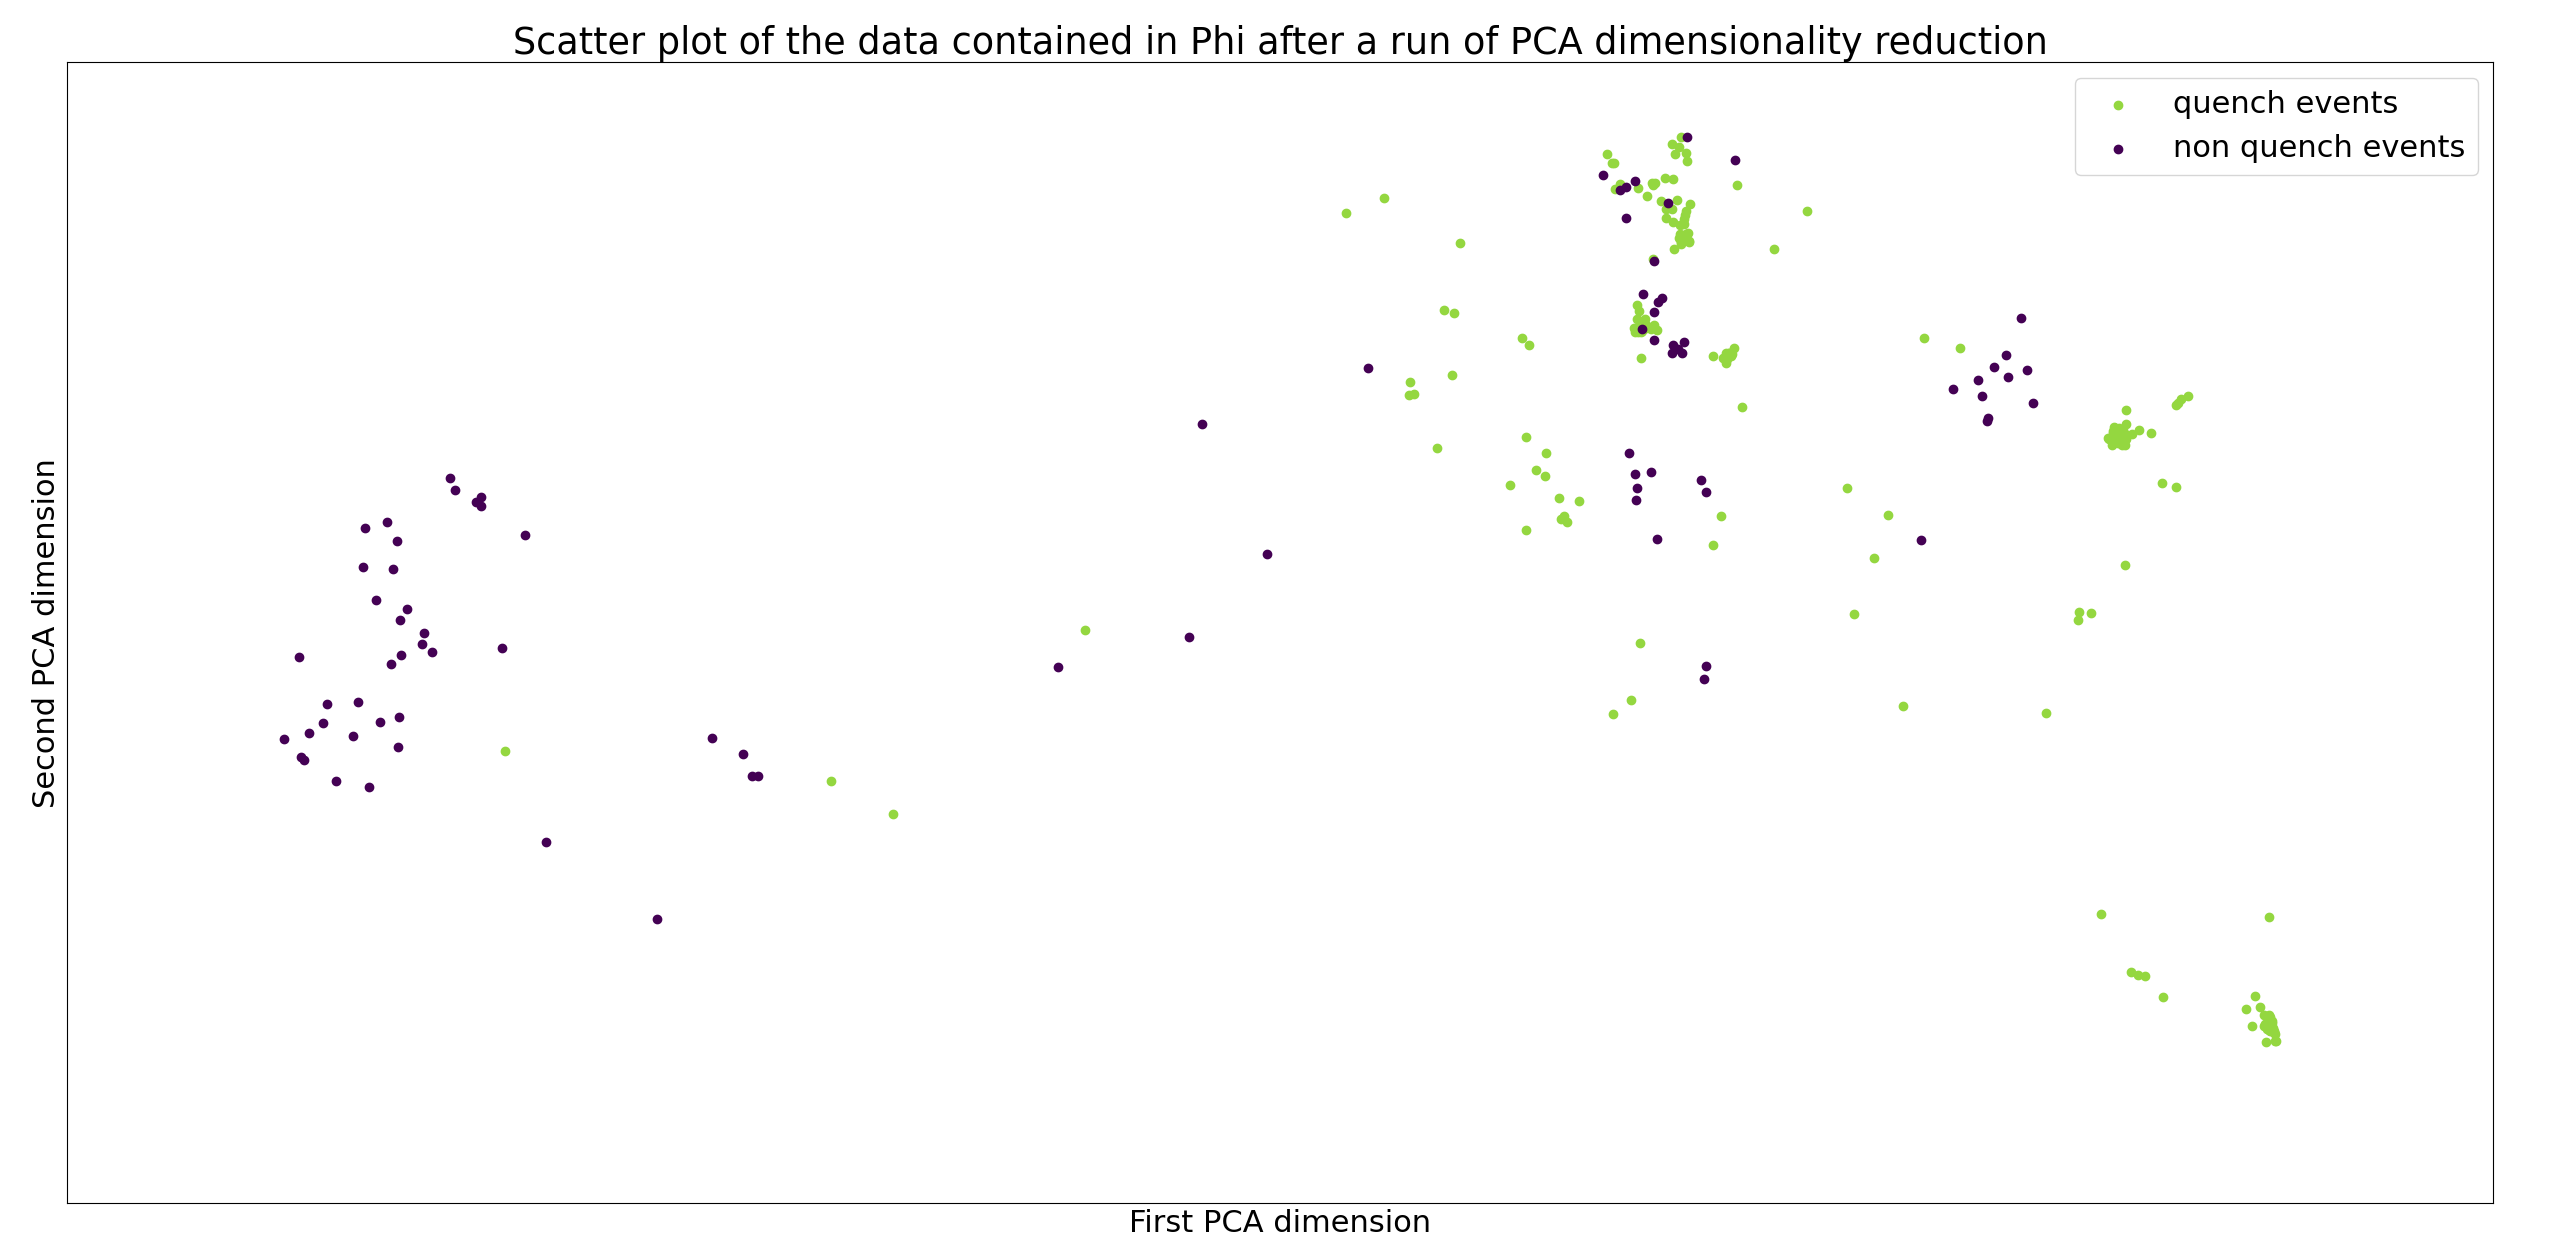
\includegraphics[width=\linewidth]{img/Phi_distribution.png}
	\caption{Data distribution for the Phi table after applying $\textsc{pca}$ dimensionality
		reduction} \label{fig:phi-dist}
\end{figure}

\medskip

As far as the correlation matrix is concerned we can see in \Cref{fig:phi-corr} that, contrarily to
the correlation matrix of other tables, the amount of harmonics that are strongly correlated with
each other is kept to a minimum. No real structure can be seen in this table as was the case of An
and Bn.
\begin{figure}[h!]
	\centering
	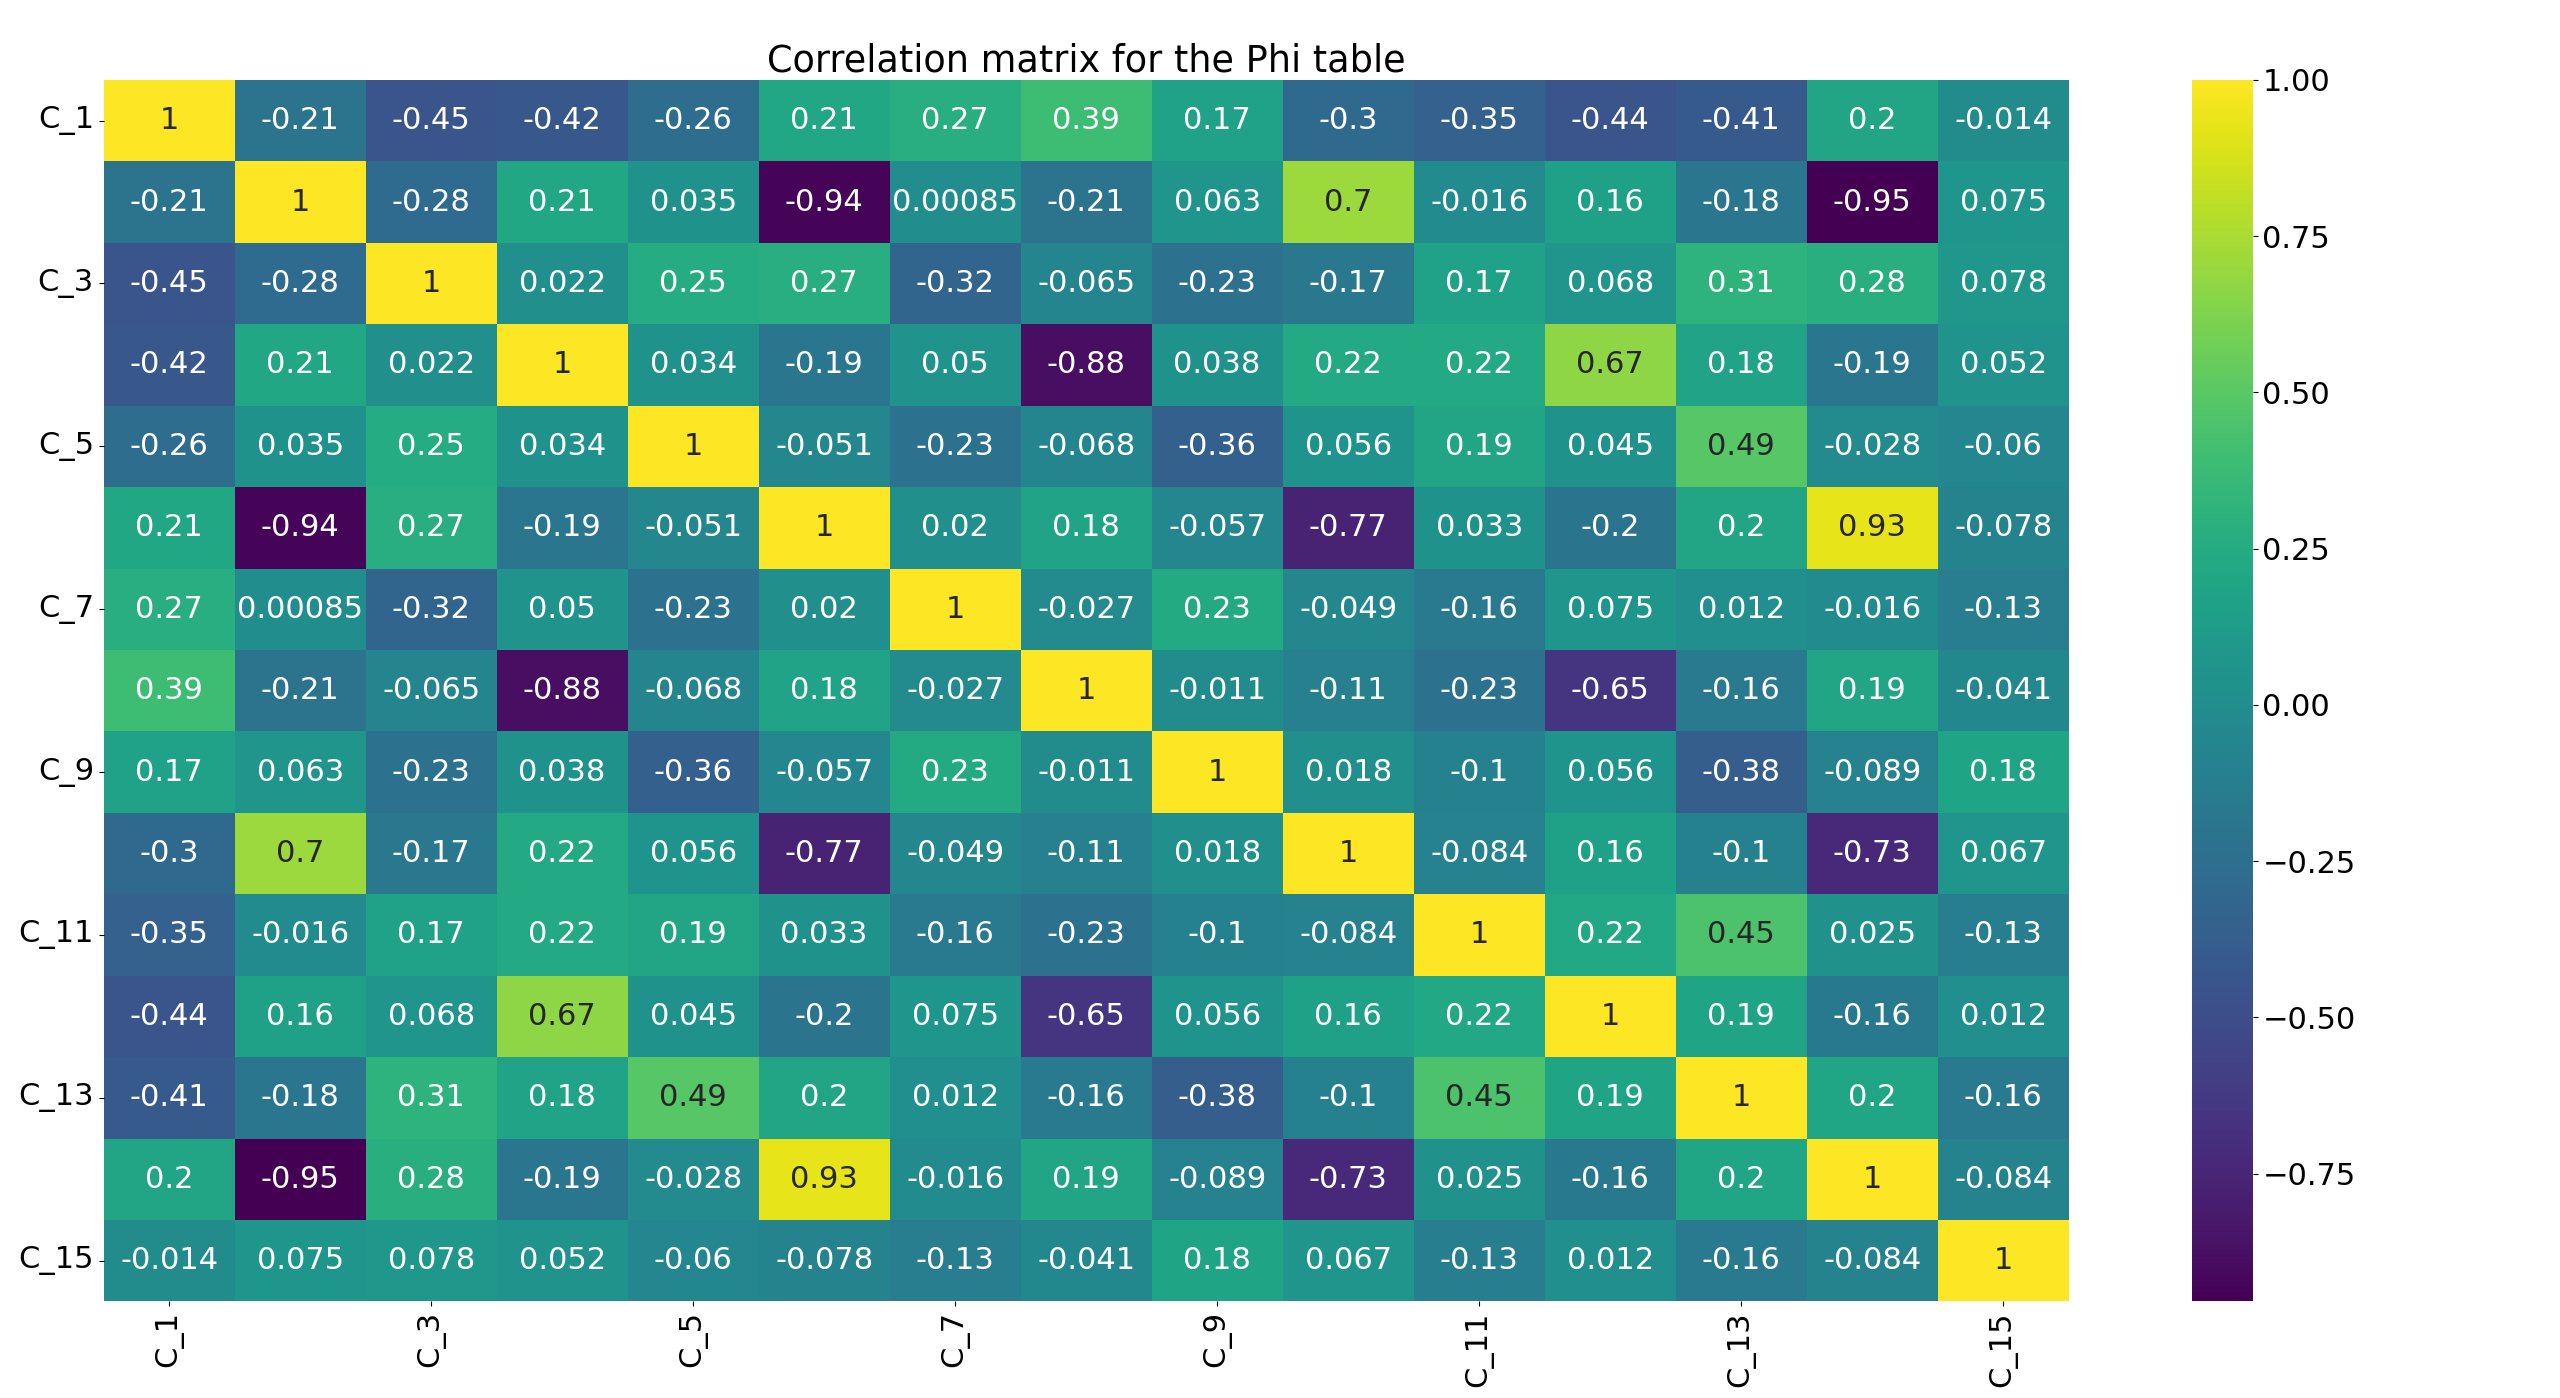
\includegraphics[width=\linewidth]{img/Phi_corr_matrix.png}
	\caption{The cross-correlation of the Phi harmonics} \label{fig:phi-corr}
\end{figure}
This structure leaves us with much more freedom as to which harmonics to pick to build datasets
(compared with An, Bn and Cnmod), the only things that really stand to the eye are that: harmonic
number $2$ is strongly correlated with its odd multiples, harmonic number $4$ is strongly correlated
with its multiples.

Lastly, we can analyze the correlation between the harmonics and the label. As we can see in \Cref{fig:phi-lcorr} most of the harmonics have a good correlation with the expected solution, especially harmonic number $2$ and its odd multiples, and harmonics number $1$ and $12$.
\begin{figure}[h!]
	\centering
	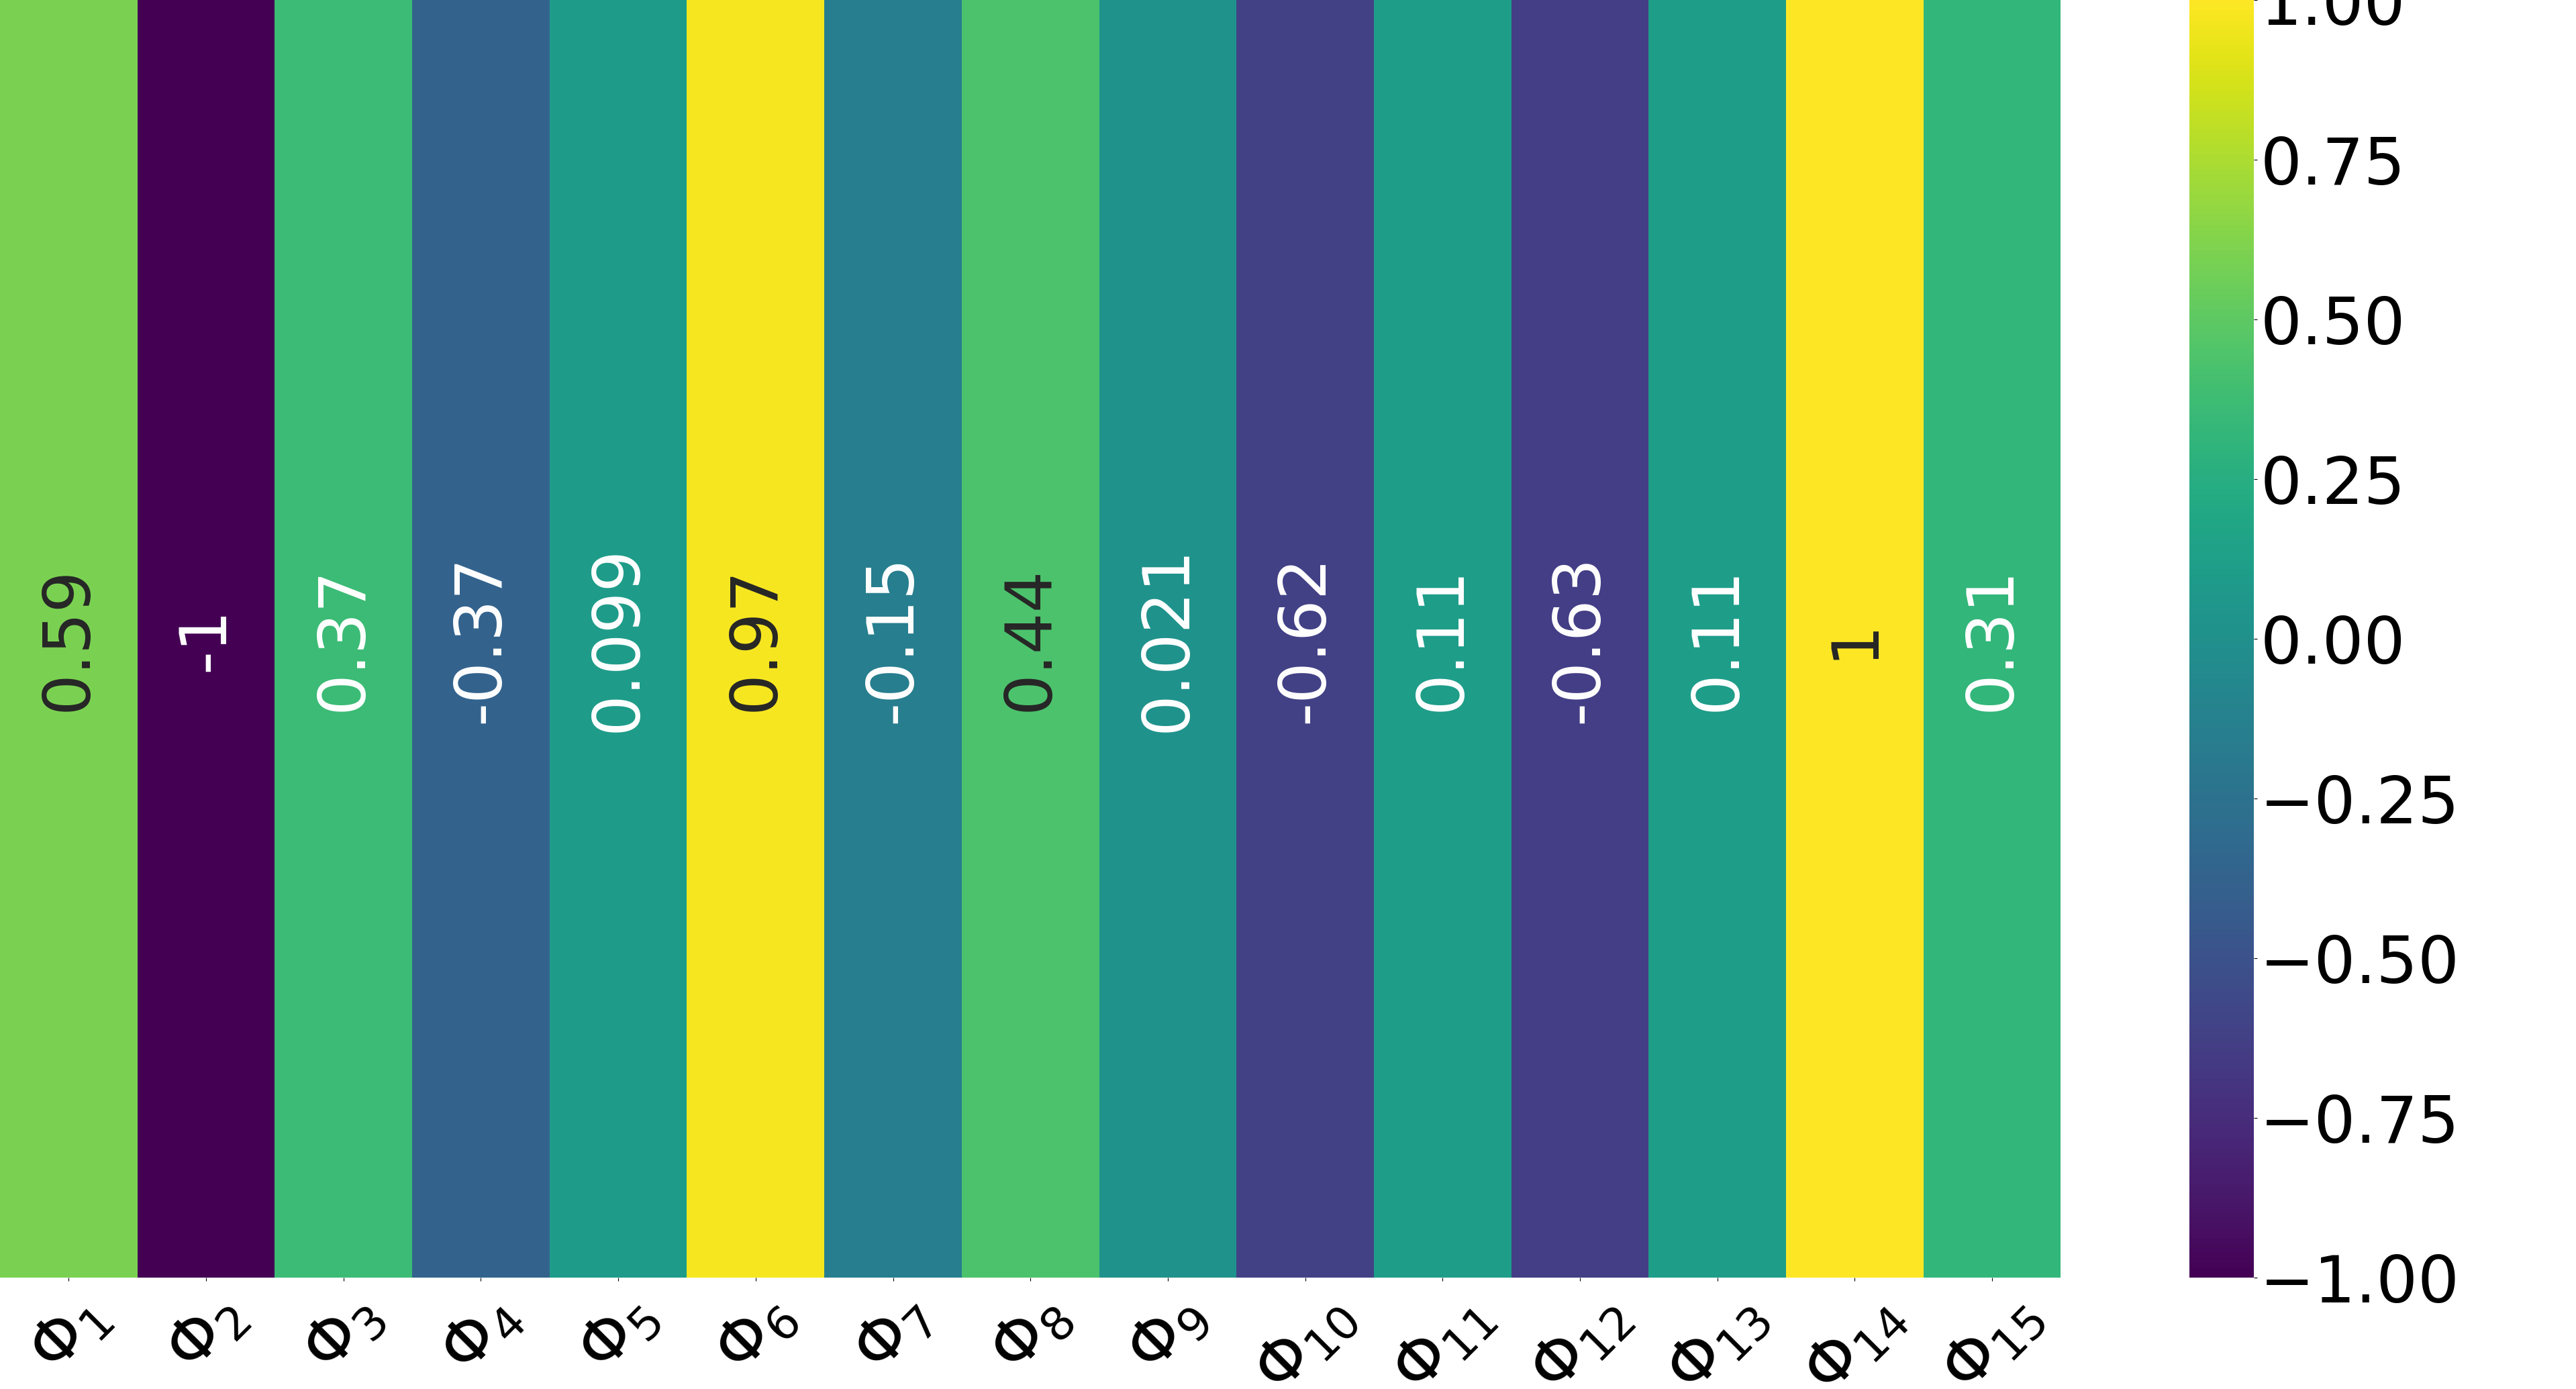
\includegraphics[width=\linewidth]{img/Phi_label_corr.png}
	\caption{Label correlation for the Phi table} \label{fig:phi-lcorr}
\end{figure}
This closes the brief exposition about the preprocessing steps for the various labels, now we will
tackle the model selection procedure indicating which were the best models overall and which model
we chose to solve $\qrp$.

\section{Results}
Every model shown in this section has been tested using the pipeline that I talked about in
\Cref{chp:problem}, due to some changes done around the time of writing, hyperparameter tuning has
been done with $\ncv$ using both the normal randomized KFold as well as StratifiedKFold. While the
performance difference is not as important as one might imagine, the final results were different
enough to push me to move the pipeline to the use of StraifiedKFold. In the following I will only
provide results for the models obtained using stratified sampling for fold construction and I will
provide a comparison of the performance metrics only when the difference is deemed appreciable.

\subsection{Decision trees}
As we already alluded to in previous sections we wanted to find a highly explainable model with good
performance that could be used to solve $\qrp$.

We tried many different approaches where various tables were involved and different harmonics were
being used, but the best table always remained An, which performance are shown in
\Cref{fig:dt-an-2-12-15-perf}. As we can see, even if we use the simple decision tree model, we are
capable of explaining whether a sample is 'quench' or 'non quench' by using a very limited amount of
harmonics (only three are necessary).
\begin{figure}
	\centering
	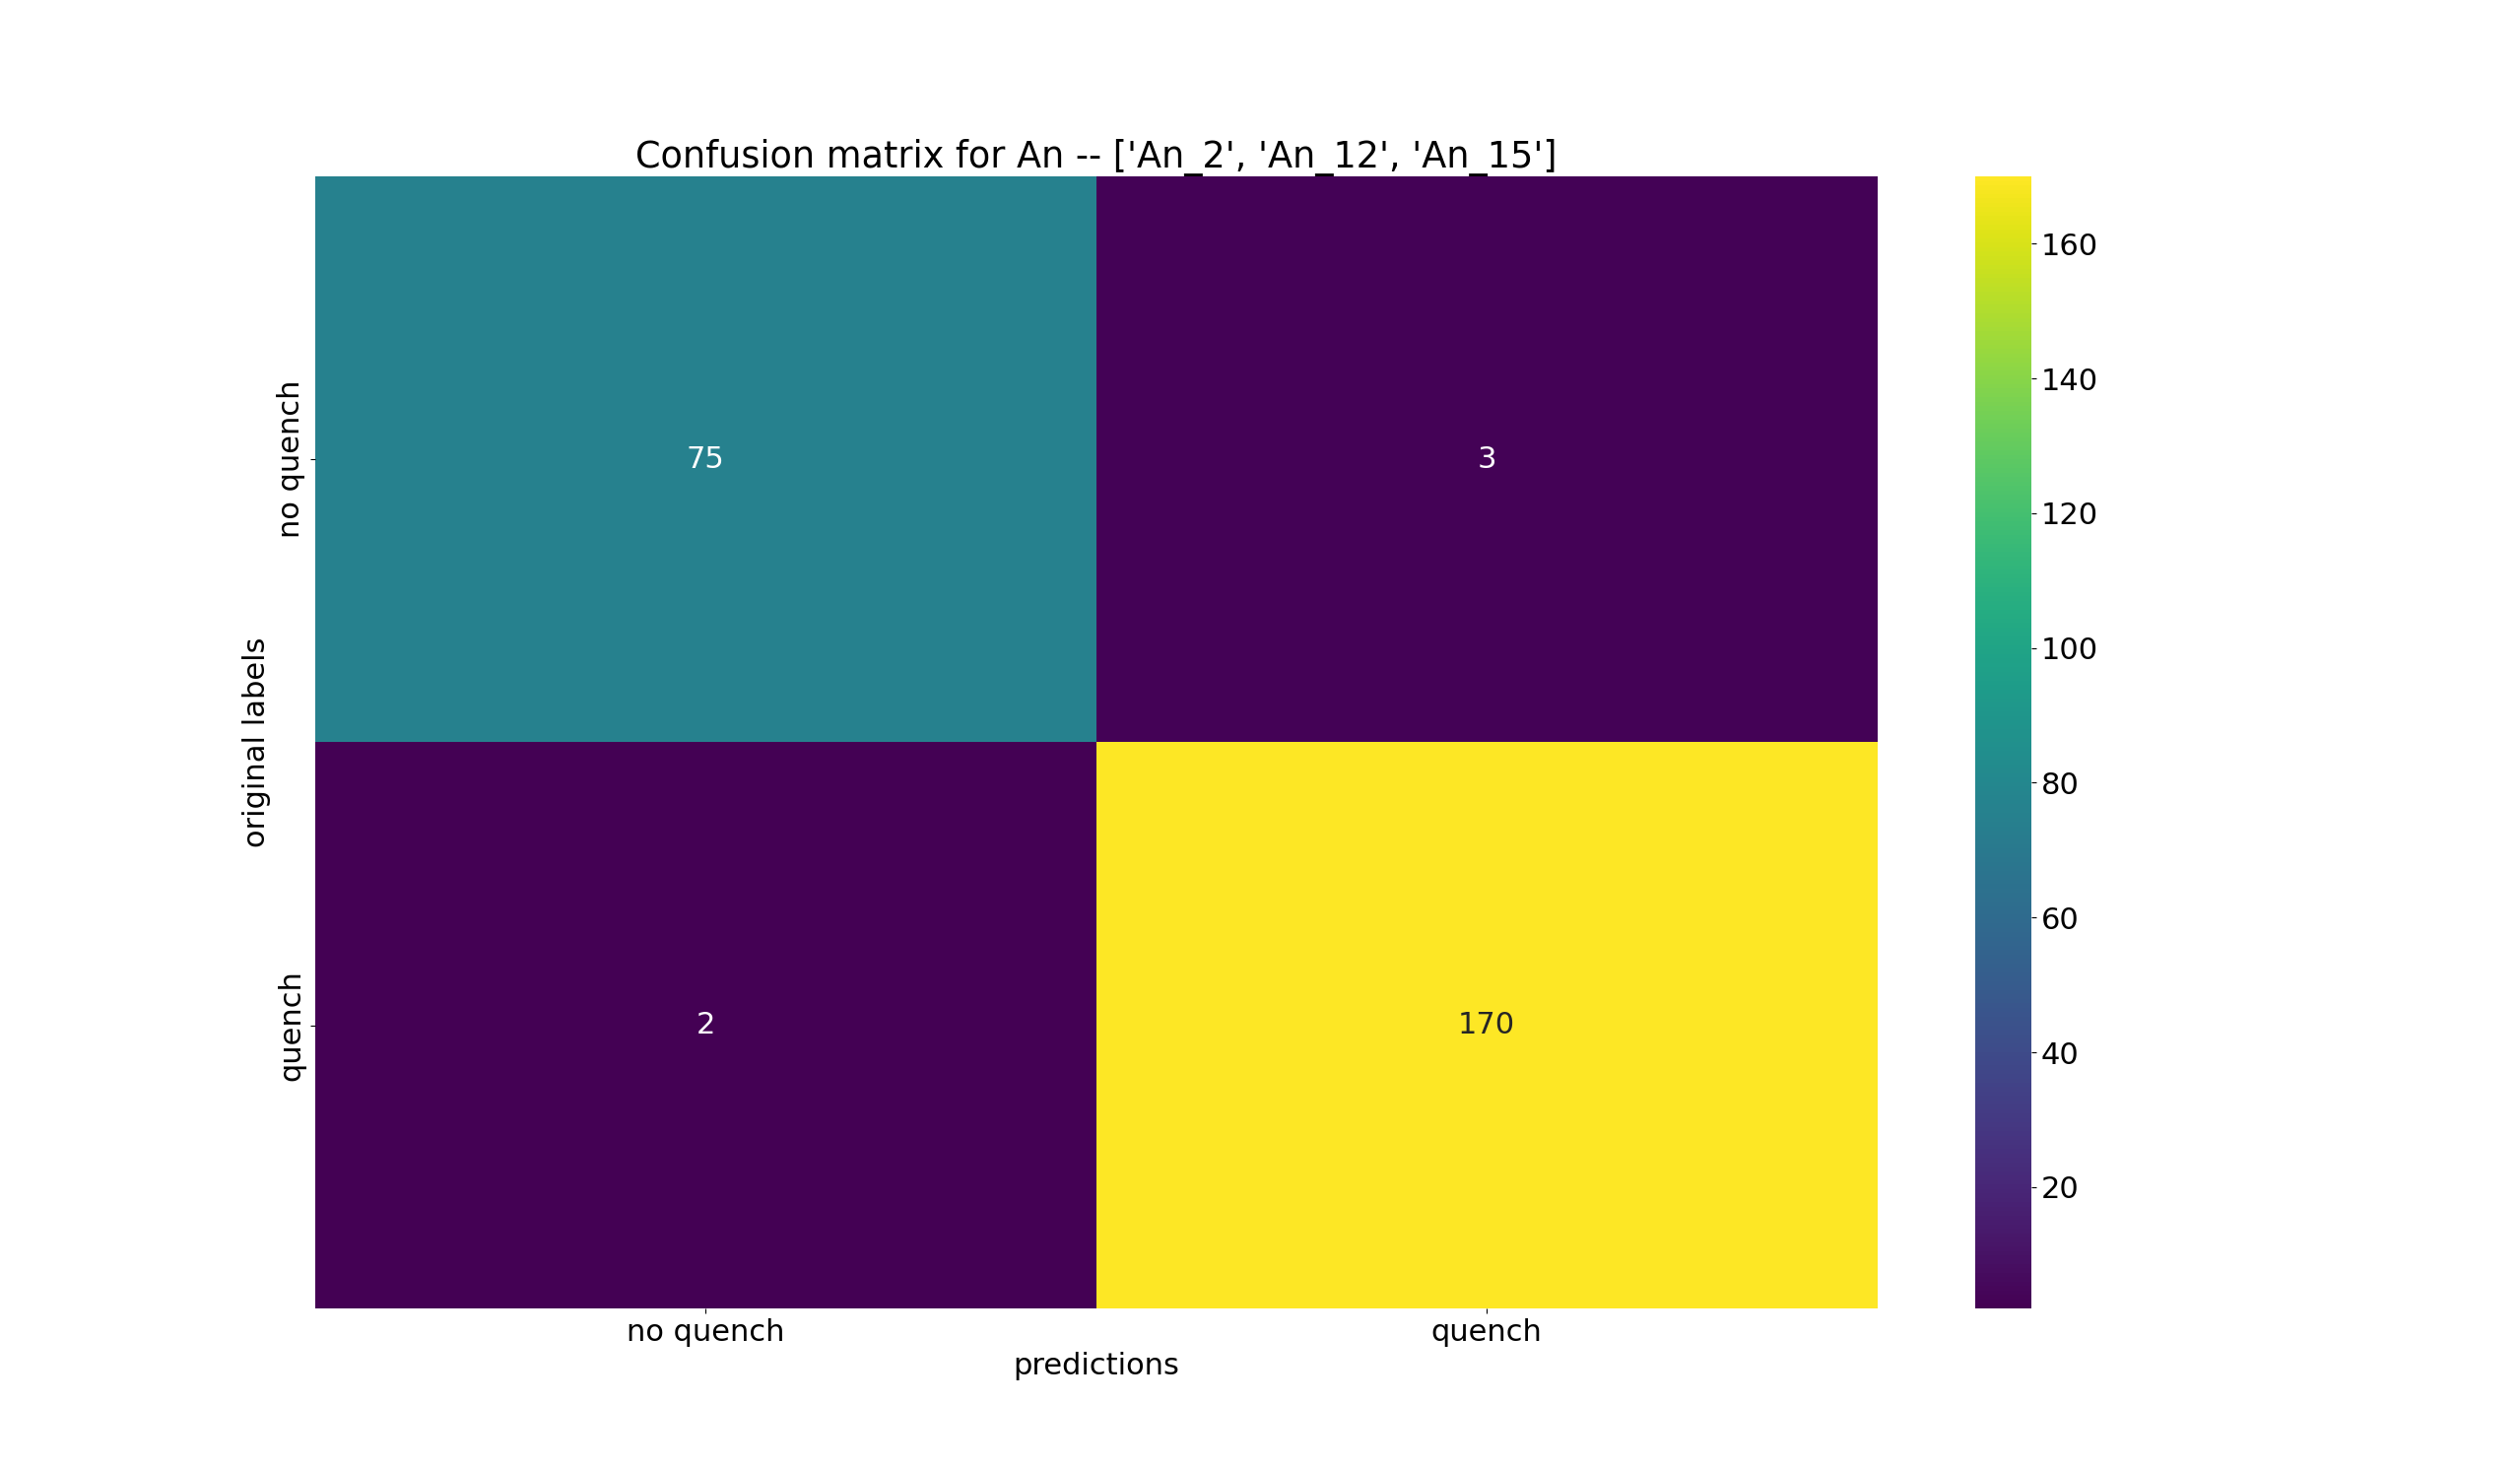
\includegraphics[width=\linewidth]{img/An_2_12_15_cm_dt.png}
	\caption{The performance for the An model built on harmonics $2, 12, 15$} \label{fig:dt-an-2-12-15-perf}
\end{figure}
If we look at \Cref{fig:dt-an-2-12-15-pt}, we can see that the structure of the tree is also
extremely simple, contained in depth, using mostly harmonic number $2$ to perform the splits and
having only one node where the impurity is not zero.
\begin{figure}
	\centering
	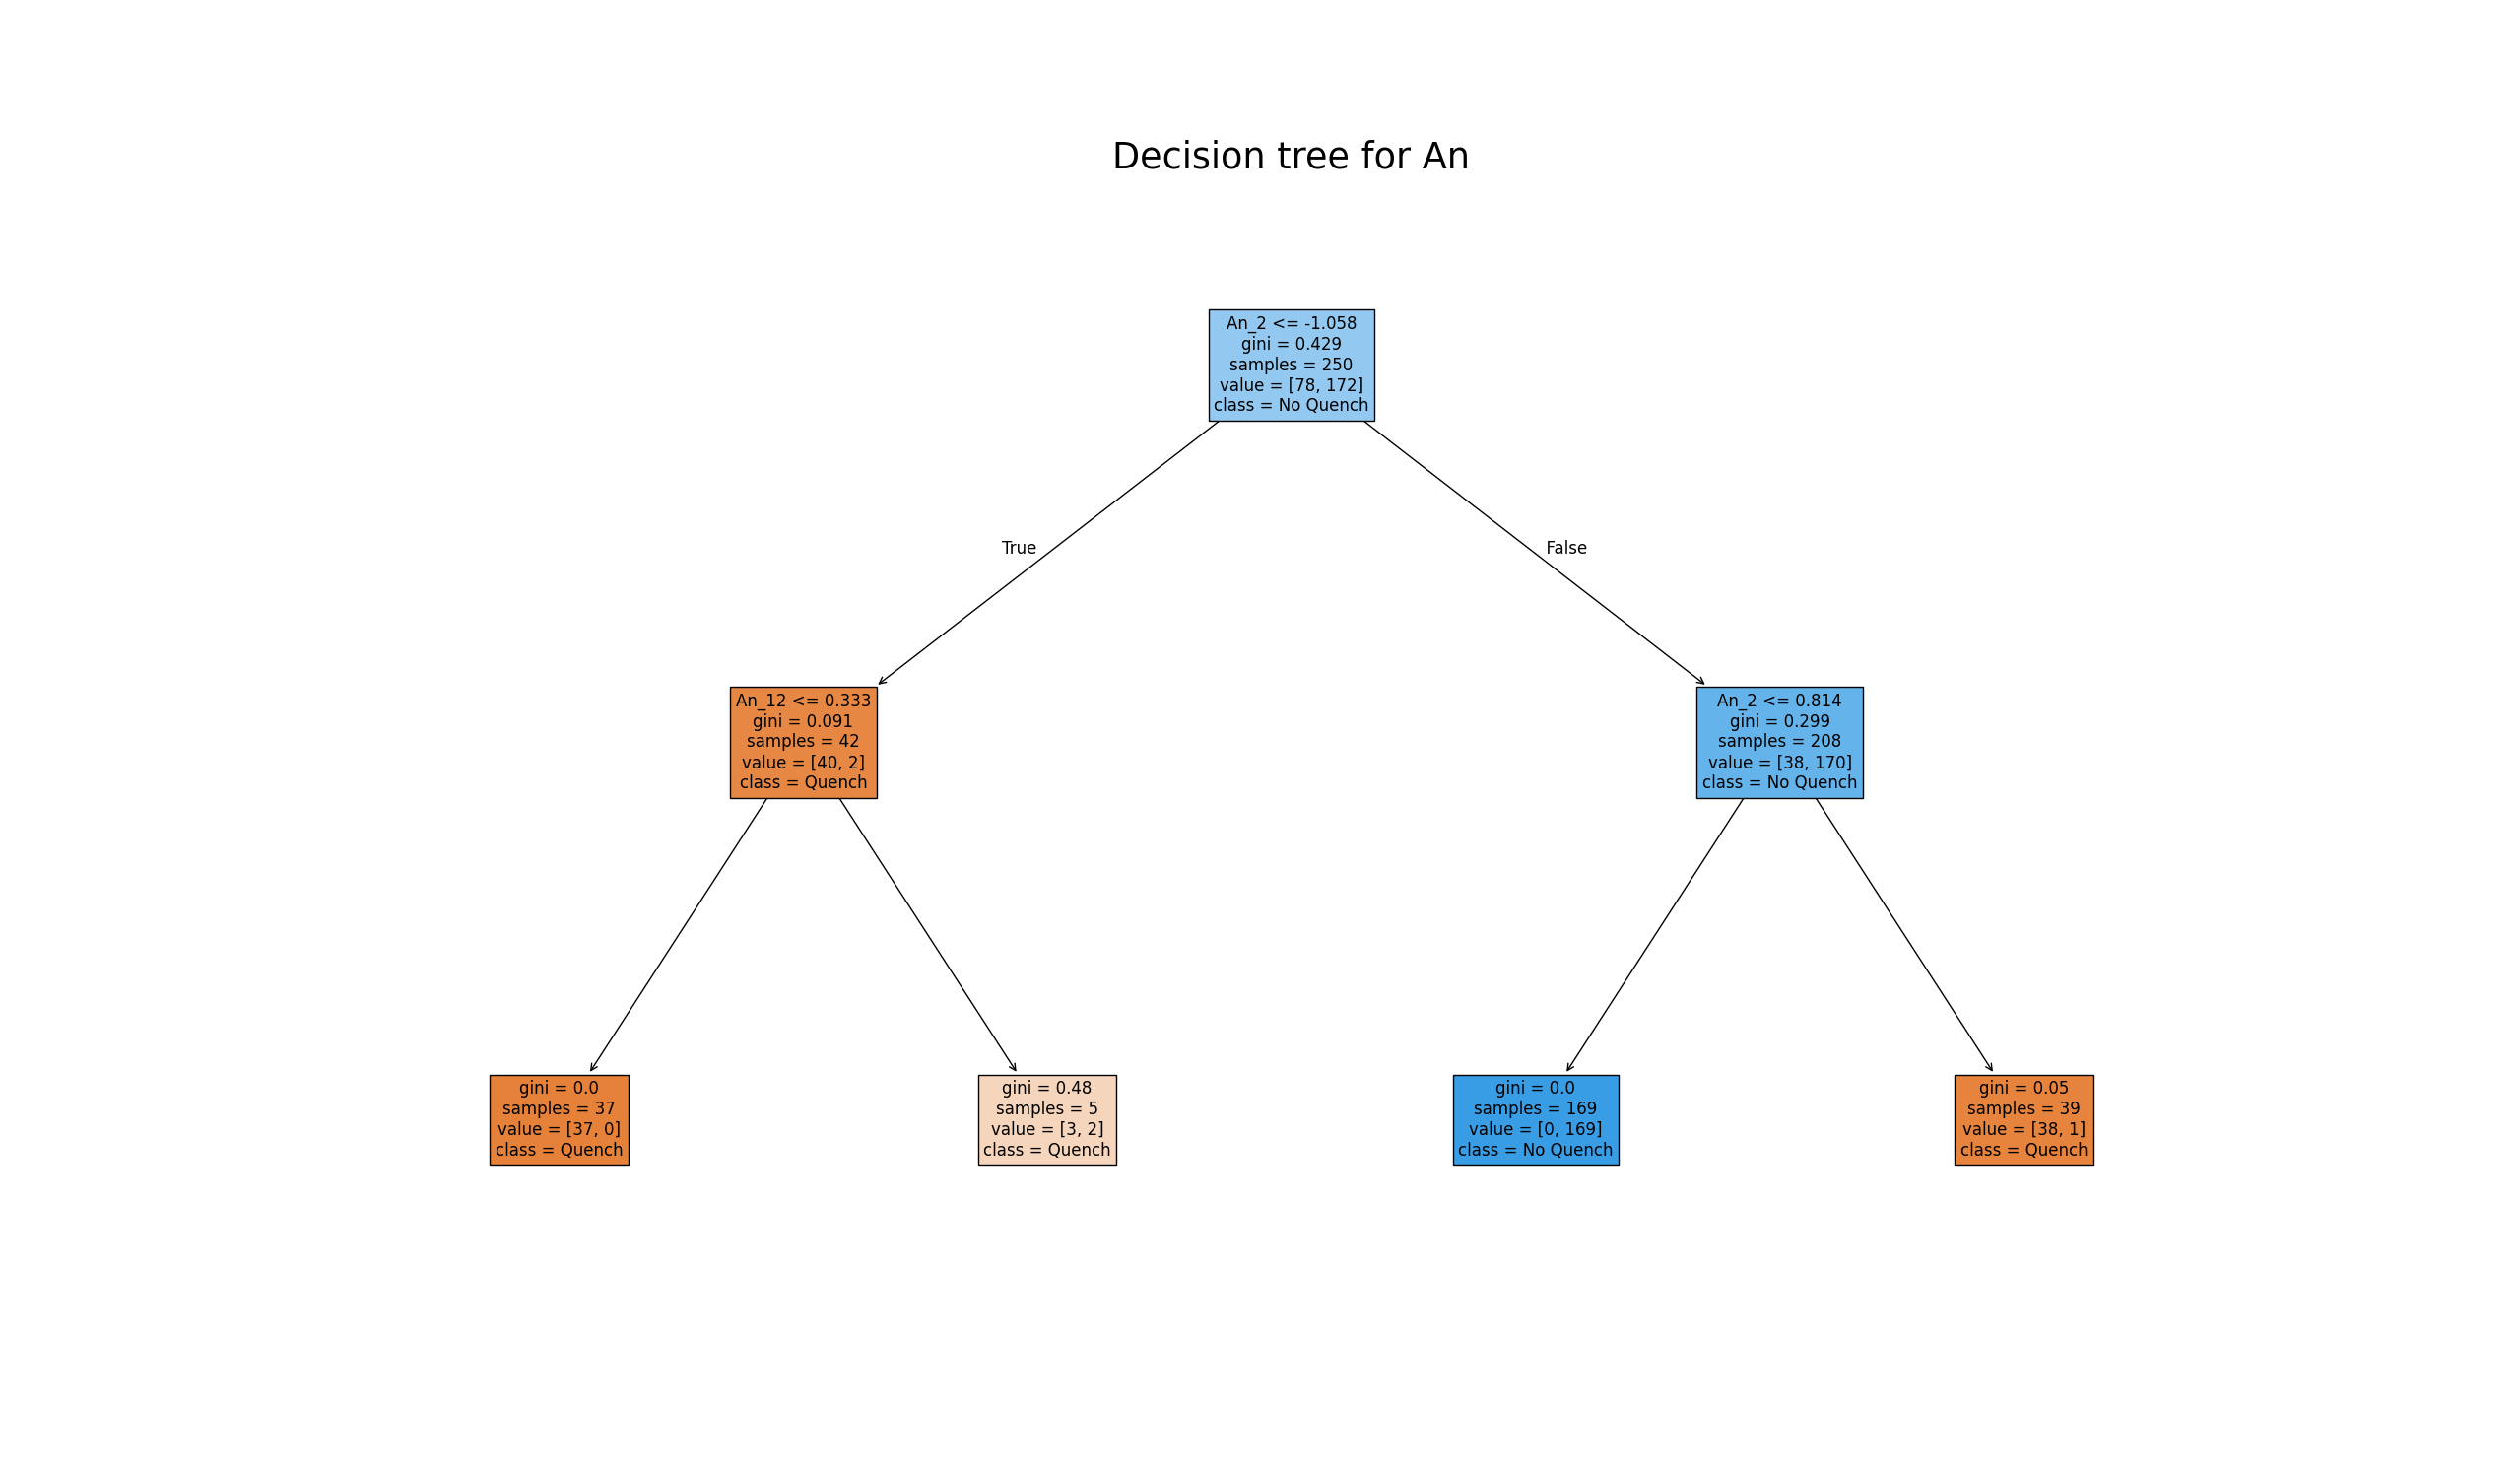
\includegraphics[width=\linewidth]{img/An_2_12_15_pt_dt.png}
	\caption{The structure of the tree built on harmonics $2, 12, 15$} \label{fig:dt-an-2-12-15-pt}
\end{figure}



